\documentclass[11pt]{article}
\usepackage[margin=1in]{geometry}
\usepackage{amsmath,amssymb,booktabs,longtable,tabularx,graphicx,float,caption,array,lmodern,pdflscape,placeins}
\usepackage[T1]{fontenc}
\usepackage{microtype}
\usepackage{hyperref}
\hypersetup{colorlinks=true,linkcolor=black,citecolor=black,urlcolor=black}
\captionsetup{font=small,labelfont=bf}
\renewcommand{\arraystretch}{1.15}
\renewcommand{\theequation}{S\arabic{equation}}
\renewcommand{\thefigure}{S\arabic{figure}}
\renewcommand{\thetable}{S\arabic{table}}
\newcommand{\ELC}{\mathrm{ELC}}
\title{Supplementary Material: An Information Theory of Extended Heredity}
\author{Nayely V\'{e}lez-Cruz and Manfred D. Laubichler}
\date{}
\begin{document}
\maketitle

\section{Overview}
To demonstrate the application of our information-theoretic framework, we constructed a simulated Extended Life Cycle (ELC) comprising $L=5$ levels of organization: a developmental gene-regulatory network, $l_{\mathrm{development}}$; a microbiome, $l_{\mathrm{microbiome}}$; a life-history process, $l_{\mathrm{life\text{-}history}}$; an epigenetic process, $l_{\mathrm{epigenetic}}$; and an ecological process, $l_{\mathrm{ecological}}$. The developmental and microbiome dynamics were based on established models of gene-regulatory networks \cite{dejong2002modeling} and microbial interactions \cite{stein2013ecological,bucci2016mdsine}, respectively. We additionally included an abiotic background process that influenced several transitions but was not itself part of the organization of the ELC, allowing us to evaluate whether the framework distinguishes hereditary factors from life-enabling background conditions. We first considered a single focal lineage $d$, treating the epigenetic state as the hereditary factor under evaluation. We quantified its predictive contribution to the next-generation ELC and its dependence on the ELC to evaluate mereological dependence, and compared these quantities with those obtained for the abiotic background process. We then extended the analysis to hereditary contributions originating from an additional parental ELC $d' \neq d$ and examined how these contributions were distributed across the levels of $d$. We next evaluated whether the epigenetic factor satisfied the criteria for a hereditary unit with respect to a focal phenotypic variant, quantified its causal specificity using Fisher information, and assessed the intergenerational stability of its hereditary contribution. We further characterized how this contribution was distributed across levels of organization and how it varied over within-generation time. Finally, we considered a configuration comprising the epigenetic and ecological factors and evaluated whether the two factors jointly satisfied the criteria for a complex unit of inheritance, including mereological dependence, synergistic information, and predictive information about the reconstruction of a focal phenotypic variant.

\section{ELC State-Space Model Architecture}
For lineage $d$, the state of level $l$ at within-level time $t_l$ is denoted by $\mathbf{x}_{d,t_l}^{[l]}$. The state-transition dynamics are given by Equation~\ref{eq:elc-state}:
\begin{equation}
\mathbf{x}_{d,t_l}^{[l]}
=
f_l\!\left(
\mathbf{A}_{d,t_l}^{[l]},
\mathbf{x}_{d,t_l-1}^{[l]},
\mathbf{C}_{d}^{[l]}
\left\{
\mathbf{x}_{d,s_{l'\to l}^{(m_{l'\to l})}(t_l)}^{[l']}
\right\}_{l' \neq l},
\sum_{d' \neq d}
B_{d,d',t_l}^{[l]}
\mathbf{x}_{d',t_l-1}^{[l]}
\right)
+
\mathbf{w}_{d,t_l-1}^{[l]} .
\label{eq:elc-state}
\end{equation}
Here, $f_l$ is the transition function for level $l$, $\mathbf{A}_{d,t_l}^{[l]}$ describes interactions among components of that level, and $\mathbf{C}_{d}^{[l]}$ maps states or trajectories from the other levels $l'\neq l$ into inputs to level $l$. For $l' \neq l$, $\mathbf{s}_{l'\to l}^{(m_{l'\to l})}(t_l)$ denotes the ordered segment of source-level $l'$ time points whose states influence the update of level $l$ at $t_l$. The term $B_{d,d',t_l}^{[l]}$ maps the state of an additional ELC $d'\neq d$ into the state transition of ELC $d$ at the same level. The vector $\mathbf{w}_{d,t_l-1}^{[l]}$ represents state-transition noise. The generation index $\tau$ is omitted from Equation~\ref{eq:elc-state} and is included in the level-specific equations below. For the focal-lineage simulation, we set all $B^{[l]}_{d,d',t_l}$ terms to zero. When considering the contributions of an additional ELC $d' \neq d$, we include a nonzero $B^{[l]}_{d,d',t_l}$ term only at the epigenetic level. The abiotic background process affects the transition equations of the five ELC levels but is not itself defined as part of the ELC. This process is denoted by $\mathbf{x}_{d,t_l}^{[l_{\mathrm{background}}]}$.

In the simulation, the transition function $f_l$ for each level is implemented by numerically integrating a stochastic differential equation over normalized within-generation time $u\in[0,1]$. The resulting trajectories are sampled at the level-specific time points $t_l$ to obtain the discrete states in Equation~\ref{eq:elc-state}. In the equations below, $du$ denotes the differential of $u$, $d\mathbf{W}$ and $dW$ denote vector-valued and scalar Brownian increments, respectively, and $\operatorname{diag}(\cdot)$ forms a diagonal matrix.

The ELC in generation $\tau$ is given by Equation~\ref{eq:sim-elc}:
\begin{equation}
\mathcal{X}^{\ELC}_{d,\tau}
=
\left\{
\mathbf{x}^{[l]}_{d,\mathcal{T}_l(\tau)}
:
l\in
\left\{
l_{\mathrm{development}},
l_{\mathrm{microbiome}},
l_{\mathrm{life\text{-}history}},
l_{\mathrm{epigenetic}},
l_{\mathrm{ecological}}
\right\}
\right\}.
\label{eq:sim-elc}
\end{equation}
Let $\mathcal{T}_l(\tau)$ denote the $T_l$ within-generation time points for level $l$ in generation $\tau$. The complete within-generation time series is given by Equation~\ref{eq:full-level-series}:
\begin{equation}
\mathbf{x}^{[l]}_{d,\mathcal{T}_l(\tau)}
=
\left(
\mathbf{x}^{[l]}_{d,t_{l,0}(\tau)},
\ldots,
\mathbf{x}^{[l]}_{d,t_{l,T_l-1}(\tau)}
\right).
\label{eq:full-level-series}
\end{equation}
For analyses that use only a portion of the complete time series, a segment of length $m_l$ is defined by Equation~\ref{eq:selected-level-segment}:
\begin{equation}
\mathbf{x}^{[l]}_{d,\mathbf{s}^{(m_l)}_l(\tau)}
=
\left(
\mathbf{x}^{[l]}_{d,t_{l,j_1}(\tau)},
\ldots,
\mathbf{x}^{[l]}_{d,t_{l,j_{m_l}}(\tau)}
\right),
\qquad
\{j_1,\ldots,j_{m_l}\}
\subsetneq
\{0,\ldots,T_l-1\}.
\label{eq:selected-level-segment}
\end{equation}
\subsection{Developmental Gene Regulatory Network Dynamics}
Gene-regulatory networks provide a standard model of developmental regulation \cite{dejong2002}. The developmental gene regulatory network (GRN) level consists of a five-node GRN representing regulatory initiation, somatic growth, stress response, maturation timing, and allocation, where the state is denoted as $\mathbf{x}^{[l_{\mathrm{development}}]}_{d,t_l(\tau)}\in\mathbb{R}^5$. The matrix $A_{\mathrm{dev}}\in\mathbb{R}^{5\times5}$ specifies the regulatory interactions among the five nodes. The term $\mathbf{C}_{d}^{[l_{\mathrm{development}}]}\{\mathbf{x}_{d,t_l(\tau)}^{[l']}\}_{l'\neq l_{\mathrm{development}}}\in\mathbb{R}^5$ represents the combined effects of the microbiome, life history, epigenetic, and ecological levels on the five developmental nodes. The vector $\mathbf{u}^{[l_{\mathrm{development}}]}_{d,t_l(\tau)}\in\mathbb{R}^5$ contains the external input to the developmental level. The vector $\boldsymbol{\sigma}_{\mathrm{dev}}\in\mathbb{R}^5$ contains the noise amplitude of each node. The developmental GRN dynamics are given by Equation~\ref{eq:development-equation}:
\begin{equation}
\begin{aligned}
d\mathbf{x}^{[l_{\mathrm{development}}]}_{d,t_l(\tau)}
&=
\Bigg[
-0.32
\mathbf{x}^{[l_{\mathrm{development}}]}_{d,t_l(\tau)}
+
1.18\tanh\!\Bigg(
A_{\mathrm{dev}}
\mathbf{x}^{[l_{\mathrm{development}}]}_{d,t_l(\tau)}
\\
&\qquad\qquad+
\mathbf{C}_{d}^{[l_{\mathrm{development}}]}
\left\{
\mathbf{x}_{d,t_l(\tau)}^{[l']}
\right\}_{l'\neq l_{\mathrm{development}}}
+
\mathbf{u}^{[l_{\mathrm{development}}]}_{d,t_l(\tau)}
\Bigg)
\Bigg]du
\\
&\quad+
\operatorname{diag}(\boldsymbol{\sigma}_{\mathrm{dev}})
d\mathbf{W}^{[l_{\mathrm{development}}]}_{d,t_l(\tau)} .
\end{aligned}
\label{eq:development-equation}
\end{equation}

\subsection{Microbiome Dynamics}
The microbiome level consists of five interacting functional groups, or microbial guilds, representing growth support, fiber fermentation, stress tolerance, opportunistic growth, and cross-feeding. Their abundances form the state $\mathbf{x}^{[l_{\mathrm{microbiome}}]}_{d,t_l(\tau)}\in\mathbb{R}_{+}^{5}$. The indices $i,j\in\{1,\ldots,5\}$ denote microbial guilds. For guild $i$, $x^{[l_{\mathrm{microbiome}}]}_{d,i,t_l(\tau)}$ is its abundance, $r_{d,i,t_l(\tau)}$ is its growth input, and $A^{\mathrm{micro}}_{ij}$ is the effect of guild $j$ on guild $i$. The growth input $r_{d,i,t_l(\tau)}$ includes effects from the developmental, epigenetic, and ecological levels and from the background process. The parameter $\sigma_{\mathrm{micro},i}$ is the noise amplitude of guild $i$. The microbiome dynamics follow a stochastic generalized Lotka-Volterra model \cite{stein2013,bucci2016} and are given by Equation~\ref{eq:microbiome-equation}:
\begin{equation}
\begin{aligned}
d\log
x^{[l_{\mathrm{microbiome}}]}_{d,i,t_l(\tau)}
&=
\left[
r_{d,i,t_l(\tau)}
+
\sum_{j=1}^{5}
A^{\mathrm{micro}}_{ij}
x^{[l_{\mathrm{microbiome}}]}_{d,j,t_l(\tau)}
-
\frac{1}{2}\sigma_{\mathrm{micro},i}^{2}
\right]du
\\
&\quad+
\sigma_{\mathrm{micro},i}
dW^{[l_{\mathrm{microbiome}}]}_{d,i,t_l(\tau)} .
\end{aligned}
\label{eq:microbiome-equation}
\end{equation}

\subsection{Life History Dynamics}
We summarize life history traits using maturation progress, growth capacity, and reproductive allocation. The life history state is $\mathbf{x}^{[l_{\mathrm{life\text{-}history}}]}_{d,t_l(\tau)}=(x_{\mathrm{mat}},x_{\mathrm{grow}},x_{\mathrm{repr}})^\top\in(0,1)^3$, where $x_{\mathrm{mat}}$ denotes maturation progress, $x_{\mathrm{grow}}$ denotes growth capacity, and $x_{\mathrm{repr}}$ denotes reproductive allocation. The indices $d$, $t_l$, and $\tau$ are omitted from the component notation for brevity. The logit transformation applied component-wise to the life history state is given by Equation~\ref{eq:logit-definition}:
\begin{equation}
\operatorname{logit}(x)
=
\log\frac{x}{1-x}.
\label{eq:logit-definition}
\end{equation}
The developmental, microbiome, epigenetic, and ecological terms in $\mathbf{U}_{d,t_l(\tau)}=(U_{\mathrm{mat}},U_{\mathrm{grow}},U_{\mathrm{repr}})^\top$ instantiate $\mathbf{C}_{d}^{[l_{\mathrm{life\text{-}history}}]}$. The functions also contain terms from the current life history state, the background process, and time $u$. Full definitions and parameter values are provided in Appendix A, \textit{Complete Equations and Parameter Values}. The life history dynamics on the logit scale are given by Equation~\ref{eq:life-equation}:
\begin{equation}
\begin{aligned}
d\,\operatorname{logit}\!\left(
\mathbf{x}^{[l_{\mathrm{life\text{-}history}}]}_{d,t_l(\tau)}
\right)
&=
2.15
\left[
\mathbf{U}_{d,t_l(\tau)}
-
\operatorname{logit}\!\left(
\mathbf{x}^{[l_{\mathrm{life\text{-}history}}]}_{d,t_l(\tau)}
\right)
\right]du
\\
&\quad+
\operatorname{diag}(0.14,0.13,0.15)
d\mathbf{W}^{[l_{\mathrm{life\text{-}history}}]}_{d,t_l(\tau)} .
\end{aligned}
\label{eq:life-equation}
\end{equation}
In Equation~\ref{eq:life-equation}, we first transform each life-history variable using the logit function. The variable increases when the resulting value is below the corresponding component of $\mathbf{U}_{d,t_l(\tau)}$ and decreases when it is above it. After each update, we apply the logistic function $\sigma(z)=1/(1+\exp(-z))$ componentwise to constrain the life-history state to $(0,1)^3$.

\subsection{Epigenetic Dynamics}
The epigenetic state is
$\mathbf{x}^{[l_{\mathrm{epigenetic}}]}_{d,t_l(\tau)}
=(x_{\mathrm{reg}},x_{\mathrm{stress}})^\top\in\mathbb{R}^2$.
The two components are abstract epigenetic state variables used to represent distinct functional roles in the simulated ELC. The regulatory variable $x_{\mathrm{reg}}$ represents epigenetic regulation of other ELC processes, whereas the stress-memory variable $x_{\mathrm{stress}}$ represents an epigenetic state that can retain the effects of prior stress-related inputs. The indices $d$, $t_l$, and $\tau$ are omitted from the component notation for brevity. When either epigenetic variable enters the dynamics of another level within the ELC, we transform its value using $\sigma(x)-0.5$, where $\sigma(x)=1/(1+\exp(-x))$. The functions $G_{\mathrm{reg},d,t_l(\tau)}$ and $G_{\mathrm{stress},d,t_l(\tau)}$ determine the values toward which the two epigenetic variables move at each point in time within a generation. These functions incorporate interactions between the two epigenetic variables together with inputs from the developmental, life-history, and ecological levels, the abiotic background process, and the normalized time variable $u$. In Equation~\ref{eq:epigenetic-equation}, the difference between each $G$ function and the current value of the corresponding epigenetic variable determines the direction and magnitude of deterministic change. The coefficients $0.92$ and $0.88$ determine the respective rates of change, while $0.24$ sets the noise amplitude for both variables. The complete definitions of the input functions and their parameter values are provided in Appendix A, \textit{Complete Equations and Parameter Values}. The epigenetic dynamics are given by Equation~\ref{eq:epigenetic-equation}:
\begin{equation}
\begin{aligned}
dx^{[l_{\mathrm{epigenetic}}]}_{d,\mathrm{reg},t_l(\tau)}
&=
0.92
\left[
G_{\mathrm{reg},d,t_l(\tau)}
-
x^{[l_{\mathrm{epigenetic}}]}_{d,\mathrm{reg},t_l(\tau)}
\right]du
+
0.24
dW^{[l_{\mathrm{epigenetic}}]}_{d,\mathrm{reg},t_l(\tau)},
\\
dx^{[l_{\mathrm{epigenetic}}]}_{d,\mathrm{stress},t_l(\tau)}
&=
0.88
\left[
G_{\mathrm{stress},d,t_l(\tau)}
-
x^{[l_{\mathrm{epigenetic}}]}_{d,\mathrm{stress},t_l(\tau)}
\right]du
+
0.24
dW^{[l_{\mathrm{epigenetic}}]}_{d,\mathrm{stress},t_l(\tau)} .
\end{aligned}
\label{eq:epigenetic-equation}
\end{equation}

\subsection{Ecological Niche Dynamics}
The ecological level models three features of the constructed niche representing the amount of organic matter in the soil, the enrichment of local food resources, and the extent to which the local environment buffers changes in temperature and moisture. These variables form the state $\mathbf{x}^{[l_{\mathrm{ecological}}]}_{d,t_l(\tau)}\in\mathbb{R}^{3}$, with the components ordered as listed above. Developmental, microbiome, and life history processes directly modify the ecological state. At the reproductive transition, components of the organism-modified ecological state contribute directly to the ecological state inherited by the next generation, representing ecological inheritance \cite{odlingsmee2003,laland2016}. The function $\mathbf{R}^{[l_{\mathrm{ecological}}]}$ describes changes produced by the current ecological state. The function $\mathbf{M}^{[l_{\mathrm{ecological}}]}$ contains inputs from the developmental, microbiome, and life history levels, the abiotic background, and time $u$. The full definitions of these functions and their parameter values are provided in Appendix A, \textit{Complete Equations and Parameter Values}. The ecological niche dynamics are given by Equation~\ref{eq:ecological-equation}:
\begin{equation}
\begin{aligned}
d\mathbf{x}^{[l_{\mathrm{ecological}}]}_{d,t_l(\tau)}
&=
\left[
\mathbf{R}^{[l_{\mathrm{ecological}}]}\!\left(
\mathbf{x}^{[l_{\mathrm{ecological}}]}_{d,t_l(\tau)}
\right)
+
\mathbf{M}^{[l_{\mathrm{ecological}}]}\!\left(
\mathcal{X}^{\ELC\setminus\{[l_{\mathrm{ecological}}]\}}_{d,\tau},
\mathbf{x}^{[l_{\mathrm{background}}]}_{d,t_l(\tau)},
u
\right)
\right]du
\\
&\quad+
\operatorname{diag}(0.13,0.13,0.12)
d\mathbf{W}^{[l_{\mathrm{ecological}}]}_{d,t_l(\tau)} .
\end{aligned}
\label{eq:ecological-equation}
\end{equation}
In Equation~\ref{eq:ecological-equation}, the values $0.13$, $0.13$, and $0.12$ are the noise amplitudes for soil organic matter, resource availability, and microclimate buffering, respectively.

\subsection{Background Process}
The background process is used to evaluate whether our framework can distinguish between life-enabling conditions and true hereditary factors and consists of a two-dimensional vector corresponding to rainfall and temperature. The state is denoted as $\mathbf{x}^{[l_{\mathrm{background}}]}_{d,t_l(\tau)}=(x^{[l_{\mathrm{background}}]}_{d,1,t_l(\tau)},x^{[l_{\mathrm{background}}]}_{d,2,t_l(\tau)})^\top\in\mathbb{R}^2$, where the first component corresponds to rainfall and the second corresponds to temperature. The background is not defined as part of the ELC, and its transition dynamics depend only on its preceding state and stochastic change. The background dynamics are given by Equation~\ref{eq:background-equation}:
\begin{equation}
\begin{aligned}
d\mathbf{x}^{[l_{\mathrm{background}}]}_{d,t_l(\tau)}
&=
\left(
-0.42
x^{[l_{\mathrm{background}}]}_{d,1,t_l(\tau)},
-0.38
x^{[l_{\mathrm{background}}]}_{d,2,t_l(\tau)}
\right)^\top du
\\
&\quad+
\operatorname{diag}(0.16,0.16)
d\mathbf{W}^{[l_{\mathrm{background}}]}_{d,t_l(\tau)} .
\end{aligned}
\label{eq:background-equation}
\end{equation}

Figure~\ref{fig:trajectories} shows the trajectories of each ELC level within a generation $\tau$, whose dynamics are given by Equations~\ref{eq:development-equation}, \ref{eq:microbiome-equation}, \ref{eq:life-equation}, \ref{eq:epigenetic-equation}, \ref{eq:ecological-equation}, and \ref{eq:background-equation}.
\begin{figure}[H]
\centering
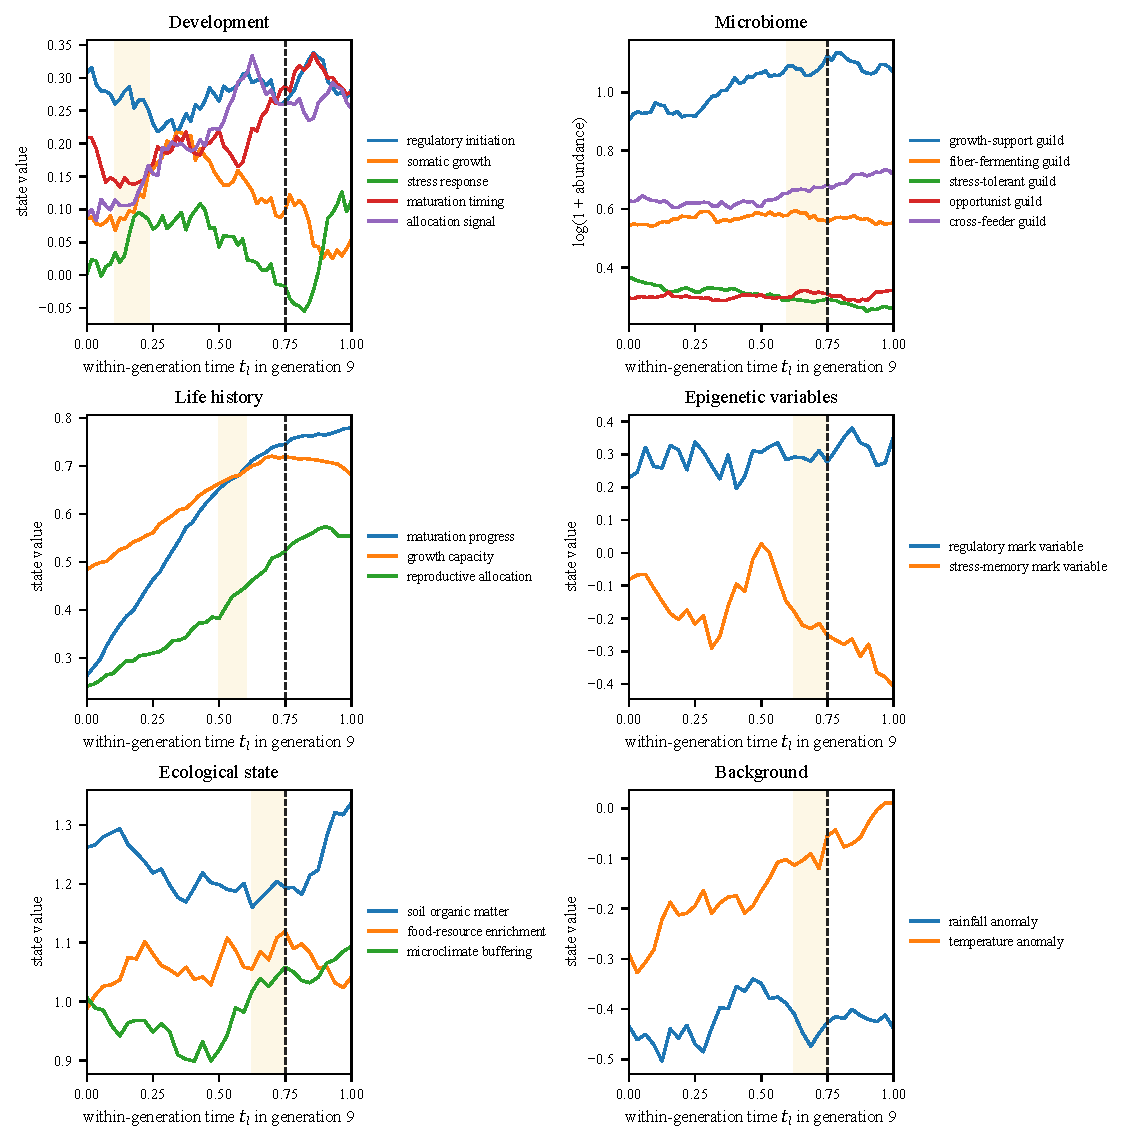
\includegraphics[width=0.98\textwidth]{figures/figure01_multilevel_dynamics.pdf}
\caption{Time series for lineage $d=1$ during generation $\tau=9$. Each panel uses the level-specific time points. The shaded interval marks the segment used in the information-theoretic analyses, and the dashed vertical line marks the reproductive transition $u_R=0.75$. Microbiome abundances are plotted as $\log(1+x)$ for visibility.}
\label{fig:trajectories}
\end{figure}

\subsection{Focal Phenotypic Variants}
We consider two focal phenotypic variants that are defined from maturation progress and growth capacity in generation $\tau+1$. We set the maturation threshold to $\theta_M=0.60$, the cutoff for early maturation to $u_{\mathrm{early}}=0.60$, and the growth threshold to $\theta_G=0.65$. The first time at which maturation progress reaches $\theta_M$ is given by Equation~\ref{eq:maturation-crossing}:
\begin{equation}
u^{\mathrm{mat}}_{d,\tau+1}
=
\min
\left\{
t_{l_{\mathrm{life\text{-}history}},j}(\tau+1)
\ \middle|\
x^{[l_{\mathrm{life\text{-}history}}]}_
{d,\mathrm{mat},
t_{l_{\mathrm{life\text{-}history}},j}(\tau+1)}
\geq
\theta_M
\right\},
\qquad
\min\varnothing=+\infty.
\label{eq:maturation-crossing}
\end{equation}
Maturation is classified as early when $u^{\mathrm{mat}}_{d,\tau+1}<u_{\mathrm{early}}$. A crossing at $u_{\mathrm{early}}$ is not classified as early. If maturation progress does not reach $\theta_M$, then $u^{\mathrm{mat}}_{d,\tau+1}=+\infty$ and maturation is classified as non-early. The phenotype variable is given by Equation~\ref{eq:phenotype-variable}:
\begin{equation}
V_{d,\tau+1}
=
\left(
\mathbf{1}
\left\{
u^{\mathrm{mat}}_{d,\tau+1}
<
u_{\mathrm{early}}
\right\},
\mathbf{1}
\left\{
x^{[l_{\mathrm{life\text{-}history}}]}_
{d,\mathrm{grow},
t_{l_{\mathrm{life\text{-}history}},
T_{l_{\mathrm{life\text{-}history}}}-1}(\tau+1)}
\geq
\theta_G
\right\}
\right).
\label{eq:phenotype-variable}
\end{equation}
In Equation~\ref{eq:phenotype-variable}, $\mathbf{1}\{\cdot\}$ denotes the indicator function. The first component of $V_{d,\tau+1}$ indicates early maturation, and the second indicates high growth at the final life history time point. Note that, $\nu=(1,1)$ denotes early maturation and high growth and $\nu=(0,0)$ denotes non-early maturation and low growth. Both components are calculated from the life history time series. Figure~\ref{fig:phenotype-reconstruction} shows the calculation of $\nu=(1,1)$ for one lineage and generation:

\begin{figure}[H]
\centering
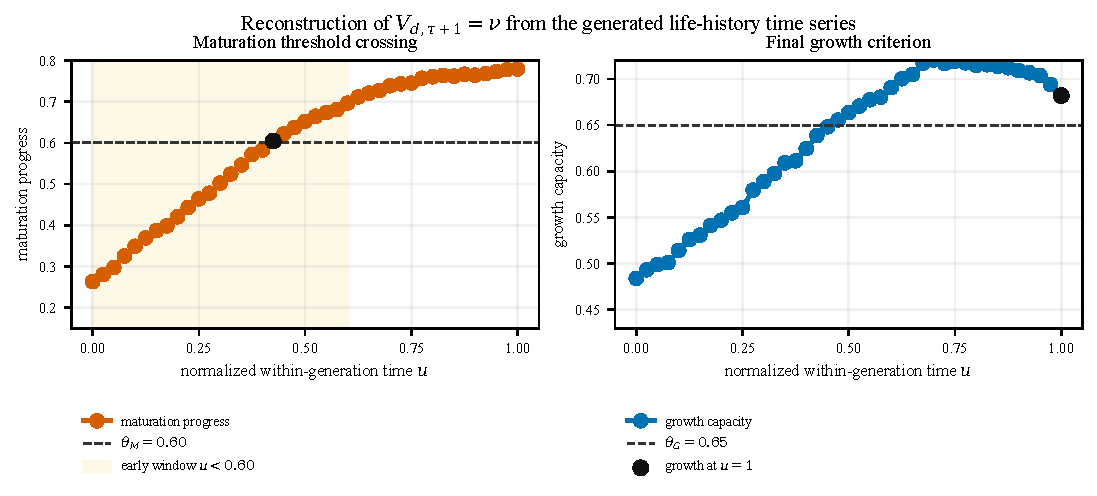
\includegraphics[width=0.92\textwidth]
{figures/figure03_phenotype_reconstruction.pdf}
\caption{Calculation of $V_{d,\tau+1}$ for lineage $d=2$ and generation $\tau+1=9$. The left panel shows maturation progress, the threshold $\theta_M=0.60$, and the first threshold crossing. The shaded interval marks $u<u_{\mathrm{early}}=0.60$. The right panel shows growth capacity at the final time point and the threshold $\theta_G=0.65$. Both conditions are satisfied, so $V_{d,\tau+1}=(1,1)$.}
\label{fig:phenotype-reconstruction}
\end{figure}
Table~\ref{tab:phenotype-distribution} reports the counts and proportions of the four phenotype states:
\begin{table}[H]
\centering
\caption{Counts and proportions of the four phenotype states across the primary simulations.}
\label{tab:phenotype-distribution}
\begin{tabular}{lrr}
\toprule
Phenotype state & Count & Proportion \\
\midrule
$(1,1)$, early maturation and high growth
& 47363 & 0.515 \\
$(1,0)$, early maturation and low growth
& 8380 & 0.0911 \\
$(0,1)$, non-early maturation and high growth
& 12298 & 0.134 \\
$(0,0)$, non-early maturation and low growth
& 23959 & 0.260 \\
\bottomrule
\end{tabular}
\end{table}

\section{Methods}
\subsection{Transfer Entropy}
Transfer entropy was estimated as conditional mutual information using a Gaussian-copula estimator \cite{schreiber2000,ince2017}. Each continuous variable was converted to Gaussian scores by ranking the observations, mapping rank $r$ among $n$ observations to $(r-0.5)/n$, and applying the inverse standard-normal distribution. The conditional mutual information was then calculated from the covariance matrix of the transformed variables and reported in bits.

\subsection{Permutation Test and Confidence Intervals}
For each information-theoretic analysis, we permuted the variable or state segment being tested across lineages within each seed and generation while keeping the target and conditioning variables fixed \cite{theiler1992}. We repeated the permutation $500$ times and defined the baseline as the mean information obtained across the permuted data sets. The percentage of the original estimate remaining after subtracting the baseline is given by Equation~\ref{eq:percent-beyond-baseline}:
\begin{equation}
100
\frac{
I-I_{\mathrm{baseline}}
}{
I
}.
\label{eq:percent-beyond-baseline}
\end{equation}
Here, $I$ is the information estimated from the original data and $I_{\mathrm{baseline}}$ is the mean information estimated from the $500$ permutations. The permutation $p$-value is given by Equation~\ref{eq:permutation-p-value}:
\begin{equation}
p_{\mathrm{perm}}
=
\frac{
1+
\#\left\{
b:
I_{\mathrm{perm}}^{(b)}
\geq
I
\right\}
}{
500+1
}.
\label{eq:permutation-p-value}
\end{equation}
In Equation~\ref{eq:permutation-p-value}, $I_{\mathrm{perm}}^{(b)}$ is the information estimated from permutation $b$. To estimate uncertainty in the transfer-entropy estimates, we generated $500$ bootstrap samples by sampling lineages with replacement \cite{efron1993,cameron2015}. Whenever a lineage was selected, all observations from that lineage were included in the bootstrap sample. The reported $95\%$ confidence intervals were calculated as the estimate plus or minus $1.96$ times the bootstrap standard error. For the partial information decomposition, we used the same procedure with $300$ bootstrap samples.

\subsection{Predicting the Reconstructed Phenotype}
To test whether a hereditary factor changes the predicted probabilities of the four possible states of $V_{d,\tau+1}$, we fit two multinomial logistic regression models. These models provided the conditional probabilities used in the subsequent information-theoretic analyses. The first model predicted $V_{d,\tau+1}$ from the ELC history after excluding the ELC level or levels being evaluated, with generation included as a categorical variable. The second model used the same inputs and also included the selected time-series data from those levels. For the epigenetic-factor analysis, this consisted of the epigenetic segment $\mathbf{x}^{[l_{\mathrm{epigenetic}}]}_{d,s_{l_{\mathrm{epigenetic}}}^{(m_{l_{\mathrm{epigenetic}}})}(\tau)}$. For the complex-unit analysis, the model included both the epigenetic and ecological segments. We applied $\ell_2$ regularization to both models, with an inverse regularization strength of $0.35$. We used five-fold cross-fitting by lineage. We divided the lineages into five folds, fit the models using four folds, and predicted the four possible states of $V_{d,\tau+1}$ for the lineages in the remaining fold. We repeated this process until every lineage had been held out once. This ensured that the probabilities used in the information-theoretic analyses for a given lineage were estimated by models that had not been fit using that lineage.

\subsection{Partial Information Decomposition}
Partial information decomposition used the Gaussian-deficiency method \cite{venkatesh2022}. The target and both sources were converted to Gaussian scores. 

\subsection{Interventions and Fisher Information}
Local changes in phenotype probabilities were estimated using central differences. For intervention coordinate $r$, the derivative for phenotype state $\nu'$ was approximated by Equation~\ref{eq:central-difference}:
\begin{equation}
\frac{
p_{\boldsymbol{\theta}_x+h\mathbf{e}_r}\left(
V_{d,\tau+1}=\nu'
\mid
\mathcal{X}^{\ELC\setminus\{[l]\},(k)}_{d,\tau}
\right)
-
p_{\boldsymbol{\theta}_x-h\mathbf{e}_r}\left(
V_{d,\tau+1}=\nu'
\mid
\mathcal{X}^{\ELC\setminus\{[l]\},(k)}_{d,\tau}
\right)
}{
2h
},
\qquad
h=0.1.
\label{eq:central-difference}
\end{equation}
In Equation~\ref{eq:central-difference}, $\mathbf{e}_r$ changes only intervention coordinate $r$. For interventions involving multiple source levels, all intervened source levels are excluded from the conditioning ELC history. The analysis used $1000$ sampled $(d,\tau)$ pairs and $1000$ simulations per pair and intervention coordinate. The same random numbers were used for the positive and negative changes. Before calculating the Fisher information matrices \cite{fisher1925,amari2016}, $0.5$ was added to each phenotype count to prevent zero probabilities and the counts were normalized.

\section{Results}

\subsection{Hereditary Information Contributed by the Epigenetic Process}
To test whether the epigenetic process contributes hereditary information, we quantified its predictive contribution to the next-generation ELC using Equation~\ref{eq:predictive-contribution-final}:
\begin{equation}
I\left(
\mathcal{X}^{\ELC\setminus\{[l]\}}_{d,\tau+1};
\mathbf{x}^{[l]}_{d,\mathbf{s}^{(m_l)}_l(\tau)}
\mid
\mathcal{X}^{\ELC\setminus\{[l]\},(k)}_{d,\tau}
\right).
\label{eq:predictive-contribution-final}
\end{equation}
For $l=l_{\mathrm{epigenetic}}$, the source is the epigenetic segment and the target is the next-generation ELC excluding the epigenetic level. The abiotic background process was evaluated using Equation~\ref{eq:background-predictive-contribution-control}:
\begin{equation}
I\left(
\mathcal{X}^{\ELC}_{d,\tau+1};
\mathbf{x}^{[l_{\mathrm{background}}]}_
{d,\mathbf{s}^{(m_{l_{\mathrm{background}}})}_{l_{\mathrm{background}}}(\tau)}
\mid
\mathcal{X}^{\ELC,(k)}_{d,\tau}
\right).
\label{eq:background-predictive-contribution-control}
\end{equation}
The epigenetic process contributed $0.201$ total bits, and $0.192$ bits beyond baseline to the next-generation ELC, compared with $0.0635$ total bits and $0.0533$ bits above baseline for the abiotic background process. The background process therefore contributed predictive information about the next-generation ELC despite not being a part of the ELC's organization. This demonstrates that predictive contribution alone is insufficient to distinguish hereditary factors from life-enabling conditions.

\subsection{Dependence of the Epigenetic Process on the ELC}
To further distinguish hereditary factors from life-enabling conditions, we tested whether the epigenetic process exhibits dependence on the ELC by quantifying the information provided by the ELC (excluding the epigenetic process in the calculations) about its future state using Equation~\ref{eq:epigenetic-closure}:
\begin{equation}
I\left(
\mathbf{x}^{[l]}_{d,\mathbf{s}^{(m_l)}_l(\tau+1)};
\mathcal{X}^{\ELC\setminus\{[l]\},(k)}_{d,\tau}
\mid
\mathbf{x}^{[l]}_{d,\mathbf{s}^{(m_l)}_l(\tau)}
\right).
\label{eq:epigenetic-closure}
\end{equation}
For $l=l_{\mathrm{epigenetic}}$, Equation~\ref{eq:epigenetic-closure} measures the information provided by the other ELC levels about the future epigenetic state after accounting for the current epigenetic state. The corresponding calculation for the background process is given by Equation~\ref{eq:background-closure-control}:
\begin{equation}
I\left(
\mathbf{x}^{[l_{\mathrm{background}}]}_
{d,\mathbf{s}^{(m_{l_{\mathrm{background}}})}_{l_{\mathrm{background}}}(\tau+1)};
\mathcal{X}^{\ELC,(k)}_{d,\tau}
\mid
\mathbf{x}^{[l_{\mathrm{background}}]}_
{d,\mathbf{s}^{(m_{l_{\mathrm{background}}})}_{l_{\mathrm{background}}}(\tau)}
\right).
\label{eq:background-closure-control}
\end{equation}

Table~\ref{tab:predictive-contribution-closure} reports the results:
\begin{table}[H]
\centering
\small
\setlength{\tabcolsep}{3pt}
\caption{Predictive contribution and dependence on the ELC.}
\label{tab:predictive-contribution-closure}
\begin{tabular}{@{}>{\raggedright\arraybackslash}p{0.20\textwidth}
>{\raggedleft\arraybackslash}p{0.10\textwidth}
>{\raggedleft\arraybackslash}p{0.13\textwidth}
>{\raggedleft\arraybackslash}p{0.13\textwidth}
>{\raggedleft\arraybackslash}p{0.11\textwidth}
>{\raggedleft\arraybackslash}p{0.15\textwidth}
>{\raggedleft\arraybackslash}p{0.07\textwidth}@{}}
\toprule
Quantity & Estimate (bits) & Baseline (bits) & Beyond baseline (bits) &
Beyond baseline (\% of estimate) & 95\% CI & $p$ \\
\midrule
Epigenetic contribution
& 0.201 & 0.00941 & 0.192 & 95.3\% & [0.196, 0.206] & 0.002 \\
Background contribution
& 0.0635 & 0.0102 & 0.0533 & 83.9\% & [0.0605, 0.0664] & 0.002 \\
Dependence of the epigenetic process on the ELC
& 0.0607 & 0.0189 & 0.0419 & 68.9\% & [0.0576, 0.0639] & 0.002 \\
Dependence of the background process on the ELC
& 0.0209 & 0.0204 & $5.30\times10^{-4}$ & 2.53\% &
[0.0187, 0.0231] & 0.194 \\
\bottomrule
\end{tabular}
\end{table}
The ELC contributed $0.0607$ total bits to the epigenetic process and $0.0419$ bits ($68.9\%$) beyond baseline. In contrast, the ELC contributed $0.0209$ total bits, or $5.30\times10^{-4}$ bits above baseline. Thus, although the background process contributed predictive information to the next-generation ELC, the ELC did not contribute predictive information to the background process. In contrast, the ELC contributed predictive information to the epigenetic process and the epigenetic process contributed predictive information to the ELC. Therefore, the epigenetic process satisfied the condition of organizational closure, whereas the background process did not. This demonstrates the ability of our framework to distinguish between true hereditary factors and life-enabling background conditions. 
Figure~\ref{fig:predictive-closure} summarizes these results:
\begin{figure}[H]
\centering
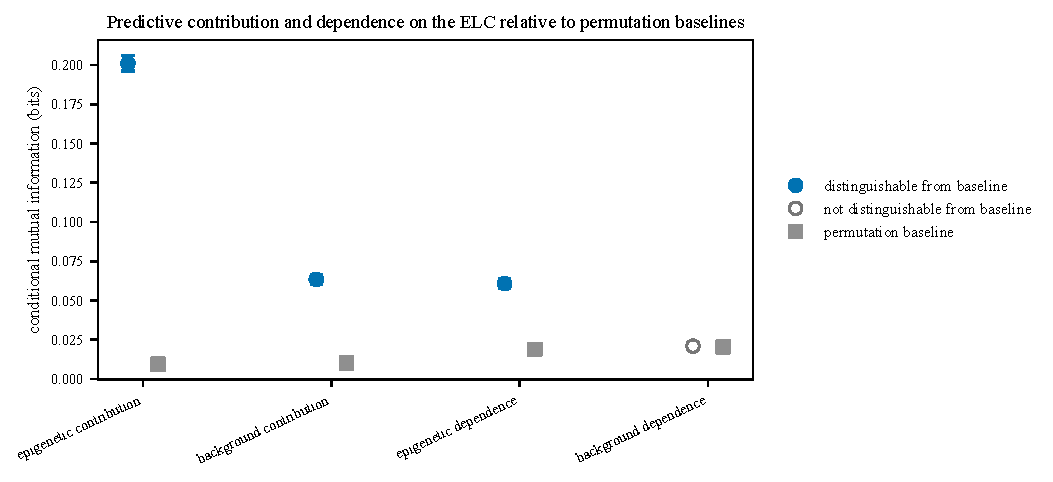
\includegraphics[width=0.86\textwidth]
{figures/figure04_predictive_contribution_closure.pdf}
\caption{Predictive contribution and dependence on the ELC. Circles show the estimates with $95\%$ confidence intervals, and squares show the means from $500$ permutations. Filled circles indicate $p\leq0.05$.}
\label{fig:predictive-closure}
\end{figure}

\subsection{Predictive Contribution from an Additional ELC}
Next, we evaluated the predictive contributions of an additional ELC $d'\neq d$  to the next-generation ELC of $d$ via Equation~\ref{eq:inter-elc-final}:
\begin{equation}
I\left(
\mathcal{X}^{\ELC}_{d,\tau+1};
\mathcal{X}^{\ELC}_{d',\tau}
\mid
\mathcal{X}^{\ELC,(k)}_{d,\tau}
\right).
\label{eq:inter-elc-final}
\end{equation}
Here, the source is the current ELC of $d'$, the target is the next-generation ELC of $d$, and the conditioning variable is the current and order-$k$ history of $d$. Furthermore, to test the contributions from individual levels of $d'$, we evaluated Equation~\ref{eq:inter-elc-source-level}:
\begin{equation}
I\left(
\mathcal{X}^{\ELC}_{d,\tau+1};
\mathbf{x}^{[l]}_{d',\mathbf{s}^{(m_l)}_l(\tau)}
\mid
\mathcal{X}^{\ELC,(k)}_{d,\tau}
\right).
\label{eq:inter-elc-source-level}
\end{equation}
Note that in our simulation, only the epigenetic level of $d'$ had a direct input to $d$, with
$B^{[l_{\mathrm{epigenetic}}]}_{d,d',t_l=0(\tau+1)}
=\operatorname{diag}(0.110,0.100)$. The $B^{[l]}$ matrices for development, microbiome, life history, and ecology were set to zero.
Table~\ref{tab:inter-elc-source} reports the predictive contributions from the complete ELC of $d'$ and its epigenetic, microbiome, and ecological levels:
\begin{table}[H]
\centering
\small
\setlength{\tabcolsep}{3pt}
\caption{Predictive contribution from the additional ELC $d'\neq d$.}
\label{tab:inter-elc-source}
\begin{tabular}{@{}>{\raggedright\arraybackslash}p{0.22\textwidth}
>{\raggedleft\arraybackslash}p{0.10\textwidth}
>{\raggedleft\arraybackslash}p{0.12\textwidth}
>{\raggedleft\arraybackslash}p{0.13\textwidth}
>{\raggedleft\arraybackslash}p{0.13\textwidth}
>{\raggedleft\arraybackslash}p{0.13\textwidth}
>{\raggedleft\arraybackslash}p{0.07\textwidth}@{}}
\toprule
Source from $d'$ & Estimate (bits) & Baseline (bits) &
Beyond baseline (bits) & Beyond baseline (\% of estimate) &
95\% CI & $p$ \\
\midrule
Complete $\mathcal{X}^{\ELC}_{d',\tau}$
& 0.146 & 0.133 & 0.0137 & 9.36\% & [0.138, 0.154] & 0.002 \\
Epigenetic segment
& 0.0252 & 0.0102 & 0.0150 & 59.5\% & [0.0233, 0.0270] & 0.002 \\
Microbiome segment
& 0.0529 & 0.0510 & 0.00186 & 3.51\% & [0.0489, 0.0568] & 0.0240 \\
Ecological segment
& 0.0171 & 0.0154 & 0.00174 & 10.2\% & [0.0152, 0.0190] & 0.002 \\
\bottomrule
\end{tabular}
\end{table}
The entire ELC of $d'$ contributed a total of $0.146$ bits and $0.0137$ bits beyond baseline to the next-generation ELC of $d$. The epigenetic segment, which is a portion of the entire epigenetic time series of $d'$, contributed a total of $0.0252$ bits and $0.0150$ bits ($59.5 \%$) beyond baseline. The microbiome and ecological segments originating from $d'$ also contributed $0.00186$ and $0.00174$ bits beyond baseline, respectively. Because the levels of $d'$ are statistically dependent, these estimates do not necessarily indicate direct microbiome or ecological inputs to $d$.

Next, we evaluated where the predictive contributions from the complete ELC of $d'$ were distributed among the levels of the next-generation ELC of $d$ via Equation~\ref{eq:inter-elc-target-level} for each level $l$:
\begin{equation}
I\left(
\mathbf{x}^{[l]}_{d,\mathbf{s}^{(m_l)}_l(\tau+1)};
\mathcal{X}^{\ELC}_{d',\tau}
\mid
\mathcal{X}^{\ELC,(k)}_{d,\tau}
\right).
\label{eq:inter-elc-target-level}
\end{equation}
To determine which levels of the next-generation ELC of $d$ receive predictive information from the epigenetic level of $d'$, we evaluated Equation~\ref{eq:inter-elc-epigenetic-target-level} for each target level $l$:
\begin{equation}
I\left(
\mathbf{x}^{[l]}_{d,\mathbf{s}^{(m_l)}_l(\tau+1)};
\mathbf{x}^{[l_{\mathrm{epigenetic}}]}_
{d',\mathbf{s}^{(m_{l_{\mathrm{epigenetic}}})}_{l_{\mathrm{epigenetic}}}(\tau)}
\mid
\mathcal{X}^{\ELC,(k)}_{d,\tau}
\right).
\label{eq:inter-elc-epigenetic-target-level}
\end{equation}

Figure~\ref{fig:inter-elc-target-profile} and Table~\ref{tab:additional-source-target-levels} summarizes the results:
\begin{figure}[H]
\centering
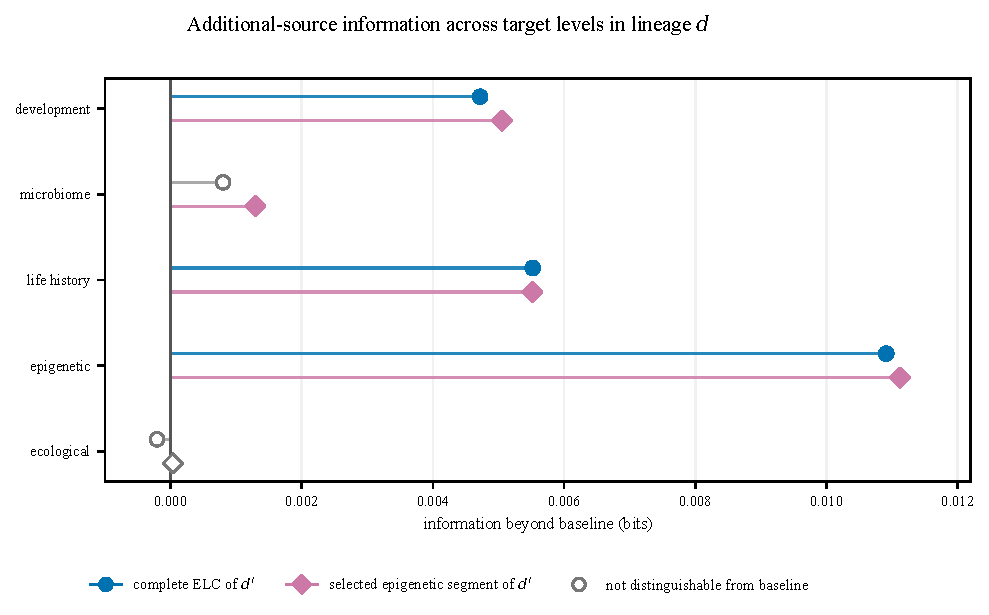
\includegraphics[width=0.90\textwidth]
{figures/figure10_inter_elc_target_profiles.pdf}
\caption{Contribution from the complete ELC of $d'$ and its epigenetic segment to each level of the next-generation ELC of $d$, after subtraction of the permutation baseline. Filled markers indicate $p\leq0.05$, and open markers indicate $p>0.05$. Values across target levels are not additive.}
\label{fig:inter-elc-target-profile}
\end{figure}

\begin{table}[H]
\centering
\small
\setlength{\tabcolsep}{4pt}
\caption{Information from the additional source lineage $d'$ about each target level in lineage $d$.}
\label{tab:additional-source-target-levels}
\begin{tabular}{lrrrrlc}
\toprule
Target level
& \shortstack{Estimate\\(bits)}
& \shortstack{Baseline\\(bits)}
& \shortstack{Beyond\\baseline (bits)}
& \shortstack{Beyond baseline\\(\% of estimate)}
& \shortstack{95\% CI\\for estimate}
& $p$\\
\midrule
\multicolumn{7}{l}{\textit{Complete ELC of $d'$}}\\
Development
& 0.0455 & 0.0408 & 0.00472 & 10.4\%
& $[0.0420,\,0.0489]$ & 0.002\\
Microbiome
& 0.0518 & 0.0510 & 0.000801 & 1.55\%
& $[0.0479,\,0.0557]$ & 0.216\\
Life history
& 0.0208 & 0.0153 & 0.00552 & 26.5\%
& $[0.0188,\,0.0228]$ & 0.002\\
Epigenetic
& 0.0212 & 0.0103 & 0.0109 & 51.5\%
& $[0.0194,\,0.0229]$ & 0.002\\
Ecological
& 0.0151 & 0.0153 & $-0.000206$ & $-1.36\%$
& $[0.0133,\,0.0170]$ & 0.687\\
\addlinespace
\multicolumn{7}{l}{\textit{Epigenetic segment of $d'$}}\\
Development
& 0.00817 & 0.00312 & 0.00505 & 61.8\%
& $[0.00711,\,0.00924]$ & 0.002\\
Microbiome
& 0.00521 & 0.00392 & 0.00130 & 24.9\%
& $[0.00428,\,0.00614]$ & 0.002\\
Life history
& 0.00668 & 0.00117 & 0.00552 & 82.5\%
& $[0.00574,\,0.00762]$ & 0.002\\
Epigenetic
& 0.0119 & 0.000794 & 0.0111 & 93.3\%
& $[0.0108,\,0.0131]$ & 0.002\\
Ecological
& 0.00122 & 0.00119 & $3.33\times10^{-5}$ & 2.73\%
& $[0.000752,\,0.00169]$ & 0.397\\
\bottomrule
\end{tabular}
\end{table}
The complete ELC of $d'$ contributed beyond baseline to the developmental, life history, and epigenetic levels of $d$, but not to the microbiome or ecological niche levels. The epigenetic segment of $d'$ contributed beyond baseline to the developmental, microbiome, life history, and epigenetic levels, but not the ecological niche level.

\subsection{Predictive Information about the Reconstruction of the Focal Variant}
To test whether the epigenetic process provides predictive information about particular phenotypes, we evaluated Equation~\ref{eq:cat-four}:
\begin{equation}
I\left(
V_{d,\tau+1};
\mathbf{x}^{[l]}_{d,\mathbf{s}^{(m_l)}_l(\tau)}
\mid
\mathcal{X}^{\ELC\setminus\{[l]\},(k)}_{d,\tau}
\right).
\label{eq:cat-four}
\end{equation}
For $l=l_{\mathrm{epigenetic}}$, Equation~\ref{eq:cat-four} measures the information provided by the epigenetic segment about the four possible states of $V_{d,\tau+1}$. For this analysis, $\nu=(1,1)$ denotes early maturation and high growth. To test whether the epigenetic process predicts $\nu$, we evaluated Equation~\ref{eq:cat-binary}:
\begin{equation}
I\left(
\mathbf{1}\left\{V_{d,\tau+1}=\nu\right\};
\mathbf{x}^{[l]}_{d,\mathbf{s}^{(m_l)}_l(\tau)}
\mid
\mathcal{X}^{\ELC\setminus\{[l]\},(k)}_{d,\tau}
\right).
\label{eq:cat-binary}
\end{equation}
The mean conditional log-ratio for $\nu$ among observations in which $\nu$ was reconstructed is given by Equation~\ref{eq:cat-log-ratio}:
\begin{equation}
\begin{aligned}
L_\nu
=
\mathbb{E}\left[
\log_2
\frac{
p\left(
V_{d,\tau+1}=\nu
\mid
\mathbf{x}^{[l]}_{d,\mathbf{s}^{(m_l)}_l(\tau)},
\mathcal{X}^{\ELC\setminus\{[l]\},(k)}_{d,\tau}
\right)
}{
p\left(
V_{d,\tau+1}=\nu
\mid
\mathcal{X}^{\ELC\setminus\{[l]\},(k)}_{d,\tau}
\right)
}
\;\middle|\;
V_{d,\tau+1}=\nu
\right].
\end{aligned}
\label{eq:cat-log-ratio}
\end{equation}
A positive value of $L_\nu$ indicates that, among cases in which $\nu$ was reconstructed, including the epigenetic segment increased the predicted probability of $\nu$ on average. Table~\ref{tab:variant-info} reports the results:
\begin{table}[H]
\centering
\small
\setlength{\tabcolsep}{3pt}
\caption{Predictive information about the reconstructed phenotype.}
\label{tab:variant-info}
\begin{tabular}{@{}>{\raggedright\arraybackslash}p{0.52\textwidth}
>{\raggedleft\arraybackslash}p{0.14\textwidth}
>{\raggedleft\arraybackslash}p{0.22\textwidth}@{}}
\toprule
Quantity & Estimate (bits) & 95\% CI \\
\midrule
Four-state phenotype
& 0.0299 & [0.0280, 0.0318] \\
Focal variant $\nu$
& 0.0212 & [0.0196, 0.0228] \\
Mean log-ratio for $\nu$
& 0.0226 & [0.0201, 0.0251] \\
\bottomrule
\end{tabular}
\end{table}
The epigenetic process transferred $0.0299$ bits about which of the four phenotype states was reconstructed and $0.0212$ bits about whether the focal variant $\nu=(1,1)$ was reconstructed. These values accounted for $2.51\%$ and $3.58\%$ of the remaining uncertainty, respectively. Among cases in which $\nu$ was reconstructed, the mean log-ratio was $0.0226$ bits, corresponding to a $1.02$-fold increase in its predicted probability. Across the $1000$ ELC contexts used in the intervention and Fisher information analyses, the epigenetic state increased the estimated probability of $\nu$ in $490$ contexts $(49.0\%)$.

\subsection{Change in the Probability of the Focal Variant After Intervention}
To test whether changing the epigenetic factor can increase the probability that $\nu$ is reconstructed, we intervened on the epigenetic state at $t_l=0$ using Equation~\ref{eq:intervention-initial-state}:
\begin{equation}
\widetilde{\mathbf{x}}^{[l_{\mathrm{epigenetic}}]}_{d,t_l=0(\tau)}(\boldsymbol{\theta}_x)
=
\mathbf{x}^{[l_{\mathrm{epigenetic}}]}_{d,t_l=0(\tau)}
+
\begin{pmatrix}
\theta_{\mathrm{reg}}\\
\theta_{\mathrm{stress}}
\end{pmatrix}.
\label{eq:intervention-initial-state}
\end{equation}
The remaining epigenetic segment was generated by the ELC dynamics. The resulting distribution over $V_{d,\tau+1}$ is given by Equation~\ref{eq:do-dist}:
\begin{equation}
\begin{aligned}
&p_{\boldsymbol{\theta}_x}\left(
V_{d,\tau+1}
\mid
\mathcal{X}^{\ELC\setminus\{[l_{\mathrm{epigenetic}}]\},(k)}_{d,\tau}
\right)
\\
&=
p\left(
V_{d,\tau+1}
\mid
\operatorname{do}\left[
\mathbf{x}^{[l_{\mathrm{epigenetic}}]}_{d,t_l=0(\tau)}
=
\widetilde{\mathbf{x}}^{[l_{\mathrm{epigenetic}}]}_{d,t_l=0(\tau)}(\boldsymbol{\theta}_x)
\right],
\mathcal{X}^{\ELC\setminus\{[l_{\mathrm{epigenetic}}]\},(k)}_{d,\tau}
\right).
\end{aligned}
\label{eq:do-dist}
\end{equation}
The remaining ELC states and the abiotic background were held at their sampled values when the intervention was applied. The model then generated the remainder of generation $\tau$ and generation $\tau+1$. The change in the probability of $\nu$ is given by Equation~\ref{eq:delta-p-nu}:
\begin{equation}
\Delta p_\nu(\boldsymbol{\theta}_x)
=
p_{\boldsymbol{\theta}_x}\left(V_{d,\tau+1}=\nu\right)
-
p_{\mathbf{0}}\left(V_{d,\tau+1}=\nu\right).
\label{eq:delta-p-nu}
\end{equation}
Table~\ref{tab:epigenetic-intervention} reports the largest increase and decrease on the tested grid:
\begin{table}[H]
\centering
\small
\setlength{\tabcolsep}{5pt}
\caption{Change in the probability of the focal variant after changing the epigenetic state.}
\label{tab:epigenetic-intervention}
\begin{tabular}{@{}>{\raggedright\arraybackslash}p{0.25\textwidth}
>{\raggedleft\arraybackslash}p{0.19\textwidth}
>{\raggedleft\arraybackslash}p{0.12\textwidth}
>{\raggedleft\arraybackslash}p{0.12\textwidth}
>{\raggedleft\arraybackslash}p{0.20\textwidth}@{}}
\toprule
Case & $(\theta_{\mathrm{reg}},\theta_{\mathrm{stress}})$ &
$p(\nu)$ & $\Delta p_\nu$ & 95\% CI for $\Delta p_\nu$ \\
\midrule
No change
& $(0,0)$ & 0.511 & 0 & -- \\
Largest increase
& $(1.5,-1.5)$ & 0.825 & 0.314 & [0.302, 0.328] \\
Largest decrease
& $(-1.5,1.5)$ & 0.182 & $-0.328$ & [$-0.340$, $-0.316$] \\
\bottomrule
\end{tabular}
\end{table}
Our results show that altering the epigenetic state to $(1.5,-1.5)$ increased the probability of $\nu$ by $0.314$, or $31.4 \%$. Changing the epigenetic state to $(-1.5,1.5)$ decreased the probability by $0.328$, or $32.8 \%$. Figure~\ref{fig:variant-intervention} shows $\Delta p_\nu$ across the tested values:
\begin{figure}[H]
\centering
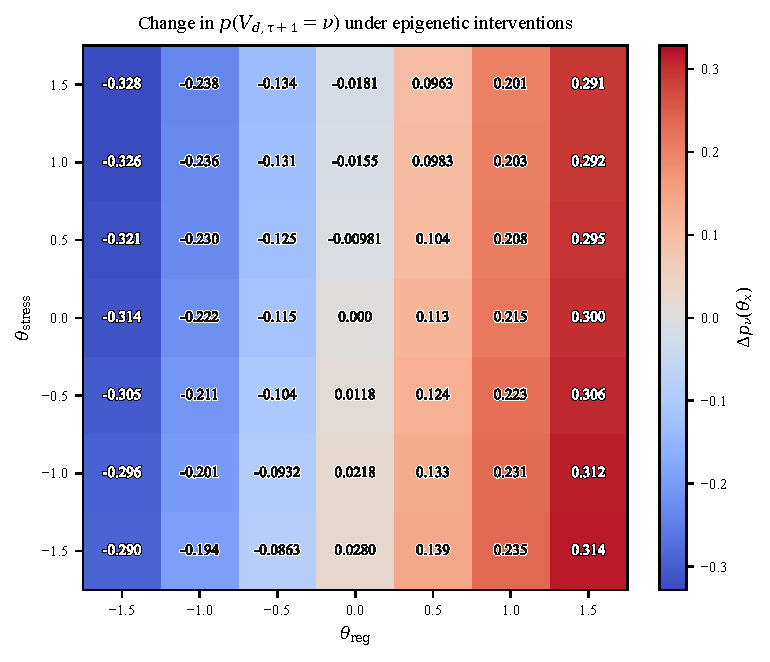
\includegraphics[width=0.82\textwidth]
{figures/figure07_epigenetic_variant_intervention_fisher.pdf}
\caption{Change in the probability of the focal variant across interventions on the epigenetic state. Positive values indicate an increase in the probability of $\nu$, and negative values indicate a decrease.}
\label{fig:variant-intervention}
\end{figure}
The local change in the probability of $\nu$ at $\boldsymbol{\theta}_x=\mathbf{0}$ is given by Equation~\ref{eq:epigenetic-local-gradient}:
\begin{equation}
\left.
\nabla_{\boldsymbol{\theta}_x}
p_{\boldsymbol{\theta}_x}\left(V_{d,\tau+1}=\nu\right)
\right|_{\boldsymbol{\theta}_x=\mathbf{0}}
=
\left(
0.233,
-0.0220
\right),
\label{eq:epigenetic-local-gradient}
\end{equation}
where the coordinates correspond to $(\theta_{\mathrm{reg}},\theta_{\mathrm{stress}})$. Increasing the regulatory epigenetic variable increased the probability of $\nu$, whereas increasing the stress-memory variable decreased the probability. The epigenetic factor therefore satisfied the criterion that an intervention can increase the probability that $\nu$ is reconstructed.

\subsection{Causal Specificity of the Epigenetic Factor}
To evaluate whether changes in the epigenetic factor alter the distribution over reconstructed phenotypes, we calculated the Fisher information matrix \cite{fisher1925,amari2016,griffiths2015,griffiths2017genetic}. For each lineage $d$ and generation $\tau$, the Fisher information matrix is given by Equation~\ref{eq:fisher-context-final}:
\begin{equation}
\mathbf{F}_x^{(d,\tau)}(\boldsymbol{\theta}_x)
=
\sum_{\nu'\in\operatorname{supp}(V_{d,\tau+1})}
\frac{
\nabla_{\boldsymbol{\theta}_x}
p_{\boldsymbol{\theta}_x}\left(
V_{d,\tau+1}=\nu'
\mid
\mathcal{X}^{\ELC\setminus\{[l]\},(k)}_{d,\tau}
\right)
\nabla_{\boldsymbol{\theta}_x}
p_{\boldsymbol{\theta}_x}\left(
V_{d,\tau+1}=\nu'
\mid
\mathcal{X}^{\ELC\setminus\{[l]\},(k)}_{d,\tau}
\right)^\top
}{
p_{\boldsymbol{\theta}_x}\left(
V_{d,\tau+1}=\nu'
\mid
\mathcal{X}^{\ELC\setminus\{[l]\},(k)}_{d,\tau}
\right)
}.
\label{eq:fisher-context-final}
\end{equation}
The remaining ELC states and the abiotic background were held fixed during each intervention. The matrix averaged across the $1000$ sampled $(d,\tau)$ pairs is given by Equation~\ref{eq:fisher-average-final}:
\begin{equation}
\overline{\mathbf{F}}_x(\boldsymbol{\theta}_x)
=
\frac{1}{1000}
\sum_{(d,\tau)\,\mathrm{sampled}}
\mathbf{F}_x^{(d,\tau)}(\boldsymbol{\theta}_x).
\label{eq:fisher-average-final}
\end{equation}
The epigenetic Fisher information matrix at $\boldsymbol{\theta}_x=\mathbf{0}$ is given by Equation~\ref{eq:epi-fisher-matrix}:
\begin{equation}
\overline{\mathbf{F}}_{\mathrm{epi}}(\mathbf{0})
=
\begin{pmatrix}
0.646 & -0.0659\\
-0.0659 & 0.0137
\end{pmatrix}.
\label{eq:epi-fisher-matrix}
\end{equation}
The coordinates are ordered as $(\theta_{\mathrm{reg}},\theta_{\mathrm{stress}})$. Both diagonal entries are positive, indicating that changes in either epigenetic coordinate alter the phenotype distribution. The larger regulatory diagonal indicates greater sensitivity to changes in the regulatory coordinate. Together with the intervention that increased the probability of $\nu$, these results support causal specificity of the epigenetic factor with respect to the reconstructed phenotype.

\subsection{Intergenerational Stability of the Epigenetic Contribution}
Next, we evaluated how many generations the epigenetic contribution persisted via Equation~\ref{eq:stability-final}:
\begin{equation}
\mathbf{R}^{[l]}_{d,\tau}(\rho)
=
\begin{pmatrix}
I\left(
\mathcal{X}^{\ELC\setminus\{[l]\}}_{d,\tau+1};
\mathbf{x}^{[l]}_{d,\mathbf{s}^{(m_l)}_l(\tau)}
\mid
\mathcal{X}^{\ELC\setminus\{[l]\},(k)}_{d,\tau}
\right)\\
I\left(
\mathcal{X}^{\ELC\setminus\{[l]\}}_{d,\tau+2};
\mathbf{x}^{[l]}_{d,\mathbf{s}^{(m_l)}_l(\tau)}
\mid
\mathcal{X}^{\ELC\setminus\{[l]\},(k)}_{d,\tau}
\right)\\
\vdots\\
I\left(
\mathcal{X}^{\ELC\setminus\{[l]\}}_{d,\tau+\rho};
\mathbf{x}^{[l]}_{d,\mathbf{s}^{(m_l)}_l(\tau)}
\mid
\mathcal{X}^{\ELC\setminus\{[l]\},(k)}_{d,\tau}
\right)
\end{pmatrix}.
\label{eq:stability-final}
\end{equation}
For $l=l_{\mathrm{epigenetic}}$, Equation~\ref{eq:stability-final} measures the contribution of the epigenetic segment in generation $\tau$ to the ELC at each future horizon. Table~\ref{tab:stability} reports the profile through $\rho=5$:
\begin{table}[H]
\centering
\small
\setlength{\tabcolsep}{4pt}
\caption{Intergenerational stability of the epigenetic contribution.}
\label{tab:stability}
\begin{tabular}{@{}>{\raggedright\arraybackslash}p{0.13\textwidth}
>{\raggedleft\arraybackslash}p{0.18\textwidth}
>{\raggedleft\arraybackslash}p{0.19\textwidth}
>{\raggedleft\arraybackslash}p{0.20\textwidth}
>{\raggedleft\arraybackslash}p{0.18\textwidth}@{}}
\toprule
Horizon $\rho$ & Estimate (bits) & Baseline (bits) &
Beyond baseline (bits) & Beyond baseline (\% of estimate) \\
\midrule
1 & 0.201 & 0.00942 & 0.192 & 95.3\% \\
2 & 0.0703 & 0.00984 & 0.0605 & 86.0\% \\
3 & 0.0382 & 0.0103 & 0.0279 & 73.1\% \\
4 & 0.0263 & 0.0108 & 0.0155 & 58.9\% \\
5 & 0.0251 & 0.0114 & 0.0137 & 54.5\% \\
\bottomrule
\end{tabular}
\end{table}
The estimated epigenetic contribution decreased from $0.201$ bits at $\rho=1$ to $0.0251$ bits at $\rho=5$. It remained distinguishable from baseline at every evaluated horizon, with $p\leq0.05$. Figure~\ref{fig:stability} shows the profile:
\begin{figure}[H]
\centering
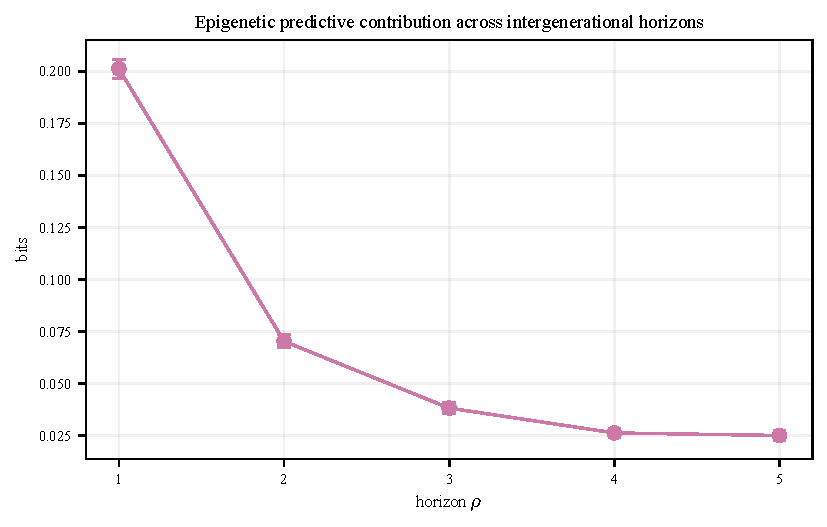
\includegraphics[width=0.72\textwidth]
{figures/figure07_intergenerational_stability.pdf}
\caption{Epigenetic contribution across five future generations. Points show the estimated information with $95\%$ confidence intervals.}
\label{fig:stability}
\end{figure}

\subsection{Location of the Predictive Contribution Across ELC Levels and Time}
Next, we evaluated how predictive information from the epigenetic factor is distributed across the levels and time points of the next-generation ELC. We evaluated Equation~\ref{eq:location-final} for each eligible target level and time with normalized time $u_{l,j}=j/(T_l-1)$ for $j=0,\ldots,T_l-1$. :
\begin{equation}
T^{[l'\to l]}_{d,\tau,t_l}
=
I\left(
\mathbf{x}^{[l]}_{d,t_l(\tau+1)};
\mathbf{x}^{[l']}_{d,\mathbf{s}^{(m_{l'})}_{l'}(\tau)}
\mid
\mathcal{X}^{\ELC\setminus\{[l']\},(k)}_{d,\tau}
\right),
\qquad
l\neq l'.
\label{eq:location-final}
\end{equation}
For $l'=l_{\mathrm{epigenetic}}$, the target levels are the developmental GRN level, microbiome level, life history level, and ecological niche level. Table~\ref{tab:location-summary} reports the maximum information beyond baseline for each target level:
\begin{table}[H]
\centering
\small
\setlength{\tabcolsep}{4pt}
\caption{Location of the epigenetic predictive contribution across ELC levels and time.}
\label{tab:location-summary}
\begin{tabular}{@{}>{\raggedright\arraybackslash}p{0.22\textwidth}
>{\raggedleft\arraybackslash}p{0.12\textwidth}
>{\raggedleft\arraybackslash}p{0.22\textwidth}
>{\raggedleft\arraybackslash}p{0.16\textwidth}
>{\raggedleft\arraybackslash}p{0.16\textwidth}@{}}
\toprule
Target level & Times & Maximum beyond baseline (bits) &
$u_{l,j}$ of maximum & Times with $p\leq0.05$ \\
\midrule
Developmental GRN level & 57 & 0.101 & 0.429 & 57/57 \\
Microbiome level & 61 & 0.0481 & 1.00 & 61/61 \\
Life history level & 41 & 0.0996 & 0.925 & 41/41 \\
Ecological niche level & 33 & 0.00117 & 1.00 & 32/33 \\
\bottomrule
\end{tabular}
\end{table}
The epigenetic contribution was greatest in the developmental GRN and life history levels and smallest in the ecological niche level. Figure~\ref{fig:location} shows the time-varying predictive contributions across the remaining ELC levels:
\begin{figure}[H]
\centering
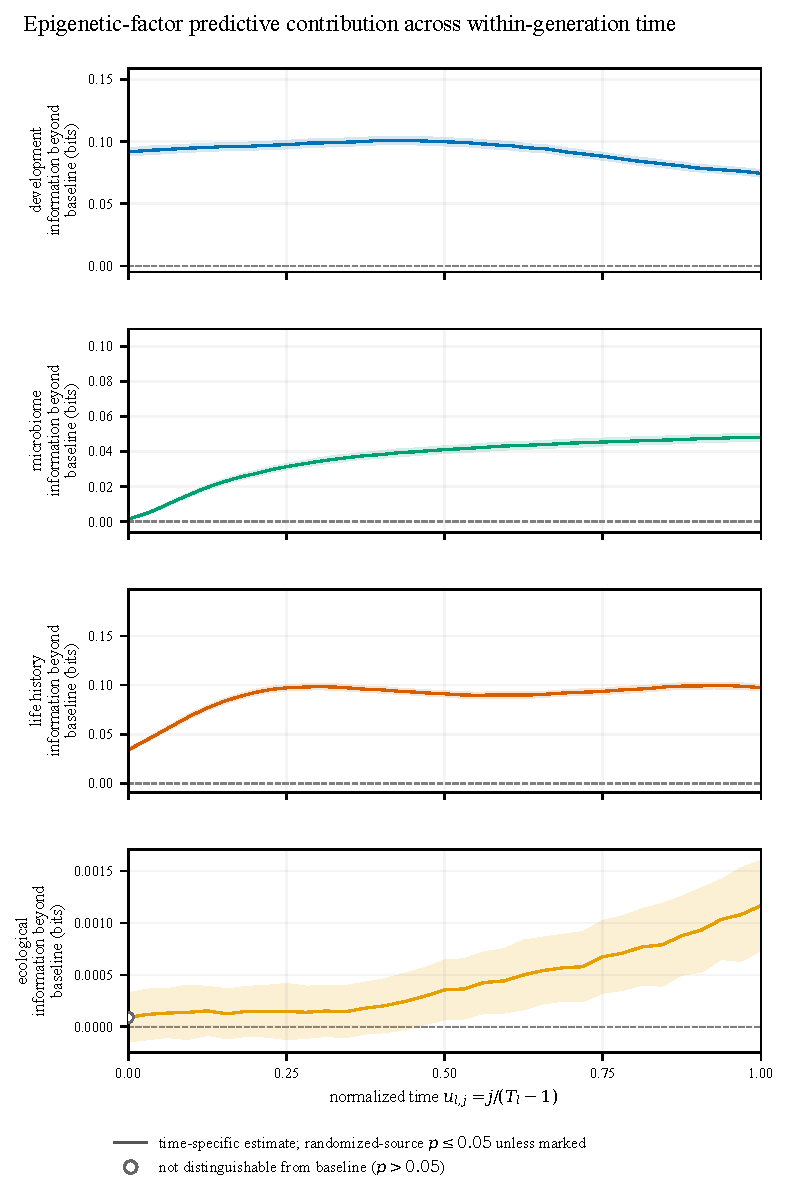
\includegraphics[width=0.58\textwidth]
{figures/figure08_level_time_location.pdf}
\caption{Epigenetic predictive contribution across normalized  time. Lines show information beyond baseline, bands show $95\%$ confidence intervals, and open markers indicate $p>0.05$.}
\label{fig:location}
\end{figure}


\subsection{Complex Units of Inheritance}
To determine whether the epigenetic and ecological factors together form a complex unit of inheritance, we first tested whether they contribute predictive information to the next-generation ELC and whether their future states depend on the ELC. We then tested whether the two factors contribute synergistic information and whether they provide predictive information about the reconstruction of $\nu$. Finally, we evaluated whether intervening on the factors can increase $p(\nu)$ and whether changes in the factors produce causally specific changes in the phenotype distribution. For this analysis, $\nu=(0,0)$ denotes non-early maturation and low growth. The epigenetic-ecological configuration is defined by Equation~\ref{eq:joint-source-definition}:
\begin{equation}
\mathbf{J}_{d,\tau}
=
\left[
\left(
\mathbf{x}^{[l_{\mathrm{epigenetic}}]}_
{d,\mathbf{s}^{(m_{l_{\mathrm{epigenetic}}})}_{l_{\mathrm{epigenetic}}}(\tau)}
\right)^\top,
\left(
\mathbf{x}^{[l_{\mathrm{ecological}}]}_
{d,\mathbf{s}^{(m_{l_{\mathrm{ecological}}})}_{l_{\mathrm{ecological}}}(\tau)}
\right)^\top
\right]^\top .
\label{eq:joint-source-definition}
\end{equation}

Its predictive contribution is given by Equation~\ref{eq:joint-predictive-contribution}:
\begin{equation}
I\left(
\mathcal{X}^{\ELC\setminus
\{[l_{\mathrm{epigenetic}}],[l_{\mathrm{ecological}}]\}}_{d,\tau+1};
\mathbf{J}_{d,\tau}
\mid
\mathcal{X}^{\ELC\setminus
\{[l_{\mathrm{epigenetic}}],[l_{\mathrm{ecological}}]\},(k)}_{d,\tau}
\right).
\label{eq:joint-predictive-contribution}
\end{equation}
Dependence of the epigenetic-ecological configuration on the ELC is given by Equation~\ref{eq:joint-predictive-closure}:
\begin{equation}
I\left(
\mathbf{J}_{d,\tau+1};
\mathcal{X}^{\ELC\setminus
\{[l_{\mathrm{epigenetic}}],[l_{\mathrm{ecological}}]\},(k)}_{d,\tau}
\mid
\mathbf{J}_{d,\tau}
\right).
\label{eq:joint-predictive-closure}
\end{equation}
The epigenetic-ecological configuration contributed $0.284$ bits beyond baseline to the next-generation ELC. The ELC provided $0.0867$ bits beyond baseline about the configuration in generation $\tau+1$. Both estimates had $p=0.002$. The epigenetic-ecological configuration therefore satisfied mereological dependence.

To determine whether the two factors contribute redundant, unique, or synergistic information, we applied the partial information decomposition in Equation~\ref{eq:pid-final}:
\begin{equation}
\begin{aligned}
&I_G\left(
\mathcal{X}^{\ELC\setminus
\{[l_{\mathrm{epigenetic}}],[l_{\mathrm{ecological}}]\}}_{d,\tau+1};
\mathbf{x}^{[l_{\mathrm{epigenetic}}]}_
{d,\mathbf{s}^{(m_{l_{\mathrm{epigenetic}}})}_{l_{\mathrm{epigenetic}}}(\tau)},
\mathbf{x}^{[l_{\mathrm{ecological}}]}_
{d,\mathbf{s}^{(m_{l_{\mathrm{ecological}}})}_{l_{\mathrm{ecological}}}(\tau)}
\mid
\mathcal{X}^{\ELC\setminus
\{[l_{\mathrm{epigenetic}}],[l_{\mathrm{ecological}}]\},(k)}_{d,\tau}
\right)
\\
&=
\operatorname{Red}
+
\operatorname{UI}_{\mathrm{epigenetic}}
+
\operatorname{UI}_{\mathrm{ecological}}
+
\operatorname{SI}.
\end{aligned}
\label{eq:pid-final}
\end{equation}
The decomposition was estimated using the Gaussian-deficiency method \cite{williams2010,bertschinger2014,venkatesh2022}. Table~\ref{tab:pid} reports the decomposition of $0.304$ bits:
\begin{table}[H]
\centering
\small
\caption{Partitioning of predictive information across the epigenetic and ecological factors.}
\label{tab:pid}
\begin{tabular}{@{}lll@{}}
\toprule
Information component & Bits & Percentage of total \\
\midrule
Redundant information & 0.0190 & 6.24\% \\
Unique epigenetic information & 0.160 & 52.6\% \\
Unique ecological information & 0.0955 & 31.4\% \\
Synergistic information & 0.0298 & 9.79\% \\
\bottomrule
\end{tabular}
\end{table}
The epigenetic factor contributed more unique information than the ecological factor. Synergistic information was $0.0298$ bits, indicating that some information was available only from the two factors together. Figure~\ref{fig:pid} shows the four PID components:
\begin{figure}[H]
\centering
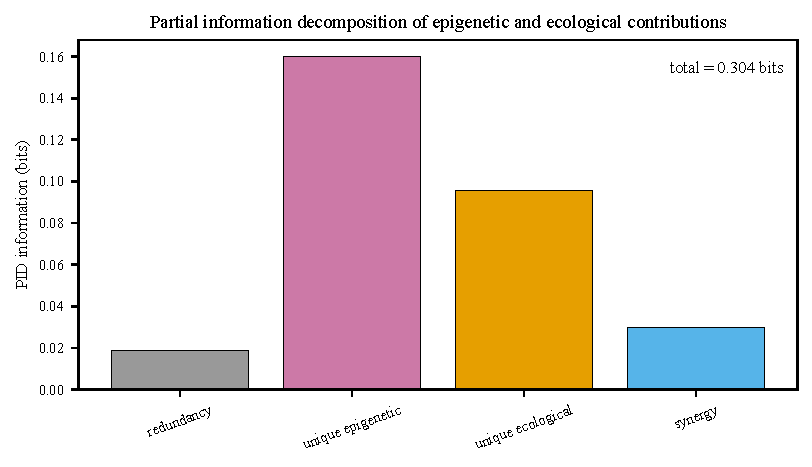
\includegraphics[width=0.62\textwidth]
{figures/figure06_epigenetic_ecological_pid.pdf}
\caption{Redundant, unique, and synergistic information contributed by the epigenetic and ecological factors. The four components sum to $0.304$ bits.}
\label{fig:pid}
\end{figure}

To determine whether the contribution to the focal phenotypic variant was irreducibly joint, we decomposed predictive information about $\nu$ using Equation~\ref{eq:joint-variant-pid}:
\begin{equation}
\begin{aligned}
&I_G\left(
\mathbf{1}\left\{V_{d,\tau+1}=\nu\right\};
\mathbf{x}^{[l_{\mathrm{epigenetic}}]}_
{d,\mathbf{s}^{(m_{l_{\mathrm{epigenetic}}})}_{l_{\mathrm{epigenetic}}}(\tau)},
\mathbf{x}^{[l_{\mathrm{ecological}}]}_
{d,\mathbf{s}^{(m_{l_{\mathrm{ecological}}})}_{l_{\mathrm{ecological}}}(\tau)}
\mid
\mathcal{X}^{\ELC\setminus
\{[l_{\mathrm{epigenetic}}],[l_{\mathrm{ecological}}]\},(k)}_{d,\tau}
\right)
\\
&=
\operatorname{Red}_{\nu}
+\operatorname{UI}_{\mathrm{epigenetic},\nu}
+\operatorname{UI}_{\mathrm{ecological},\nu}
+\operatorname{SI}_{\nu}.
\end{aligned}
\label{eq:joint-variant-pid}
\end{equation}
The Gaussian-deficiency PID decomposed $0.0270$ bits, as reported in Table~\ref{tab:joint-variant-pid}:
\begin{table}[H]
\centering
\small
\caption{Partitioning of predictive information about $\nu=(0,0)$.}
\label{tab:joint-variant-pid}
\begin{tabular}{@{}lll@{}}
\toprule
Information component & Bits & Percentage of total \\
\midrule
Redundant information & 0.00792 & 29.3\% \\
Unique epigenetic information & 0.00807 & 29.9\% \\
Unique ecological information & 0.000 & 0.0\% \\
Synergistic information & 0.0110 & 40.8\% \\
\bottomrule
\end{tabular}
\end{table}
Synergistic information about $\nu$ was $0.0110$ bits, with a $95\%$ confidence interval of $[0.00982,0.0122]$, demonstrating that part of the predictive information about the reconstruction of $\nu$ was available only from the epigenetic and ecological factors together. Figure~\ref{fig:joint-variant-pid} shows the four components:
\begin{figure}[H]
\centering
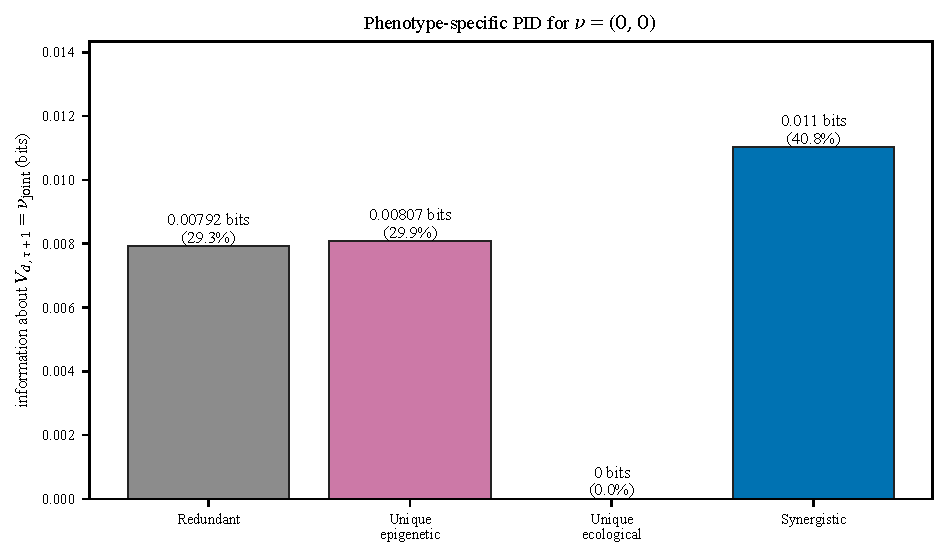
\includegraphics[width=0.62\textwidth]
{figures/figure11_joint_variant_00_pid.pdf}
\caption{Redundant, unique, and synergistic information about $\nu=(0,0)$. The four components sum to $0.0270$ bits.}
\label{fig:joint-variant-pid}
\end{figure}

We also evaluated how predictive information from the epigenetic-ecological configuration is distributed across the remaining levels of the next-generation ELC using Equation~\ref{eq:joint-location-final}:
\begin{equation}
\begin{aligned}
T^{[\mathrm{epi+eco}\to l]}_{d,\tau,t_l}
&=
I\left(
\mathbf{x}^{[l]}_{d,t_l(\tau+1)};
\mathbf{x}^{[l_{\mathrm{epigenetic}}]}_
{d,\mathbf{s}^{(m_{l_{\mathrm{epigenetic}}})}_{l_{\mathrm{epigenetic}}}(\tau)},
\mathbf{x}^{[l_{\mathrm{ecological}}]}_
{d,\mathbf{s}^{(m_{l_{\mathrm{ecological}}})}_{l_{\mathrm{ecological}}}(\tau)}
\mid
\mathcal{X}^{\ELC\setminus
\{[l_{\mathrm{epigenetic}}],[l_{\mathrm{ecological}}]\},(k)}_{d,\tau}
\right),
\\[-0.2em]
&\qquad
l\notin
\{l_{\mathrm{epigenetic}},l_{\mathrm{ecological}}\}.
\end{aligned}
\label{eq:joint-location-final}
\end{equation}
The target levels are the developmental GRN level, microbiome level, and life history level. Table~\ref{tab:joint-location-summary} reports the maximum information beyond baseline for each target level:
\begin{table}[H]
\centering
\small
\setlength{\tabcolsep}{2.5pt}
\caption{Location of the predictive contribution of the epigenetic-ecological configuration across ELC levels and time.}
\label{tab:joint-location-summary}
\begin{tabular}{@{}
>{\raggedright\arraybackslash}p{0.18\textwidth}
>{\raggedleft\arraybackslash}p{0.05\textwidth}
>{\raggedleft\arraybackslash}p{0.13\textwidth}
>{\raggedleft\arraybackslash}p{0.15\textwidth}
>{\raggedleft\arraybackslash}p{0.13\textwidth}
>{\raggedleft\arraybackslash}p{0.10\textwidth}
>{\raggedleft\arraybackslash}p{0.12\textwidth}@{}}
\toprule
Target level
& Times
& Estimated information at maximum (bits)
& Beyond baseline at maximum (bits)
& Beyond baseline (\% of estimate)
& $u_{l,j}$ of maximum
& Times with $p\leq0.05$ \\
\midrule
Developmental GRN level
& 57 & 0.150 & 0.149 & 99.3\% & 0.464 & 57/57 \\
Microbiome level
& 61 & 0.102 & 0.101 & 99.0\% & 1.00 & 61/61 \\
Life history level
& 41 & 0.184 & 0.183 & 99.7\% & 0.950 & 41/41 \\
\bottomrule
\end{tabular}
\end{table}
Figure~\ref{fig:joint-location} shows the time-varying contributions:
\begin{figure}[H]
\centering
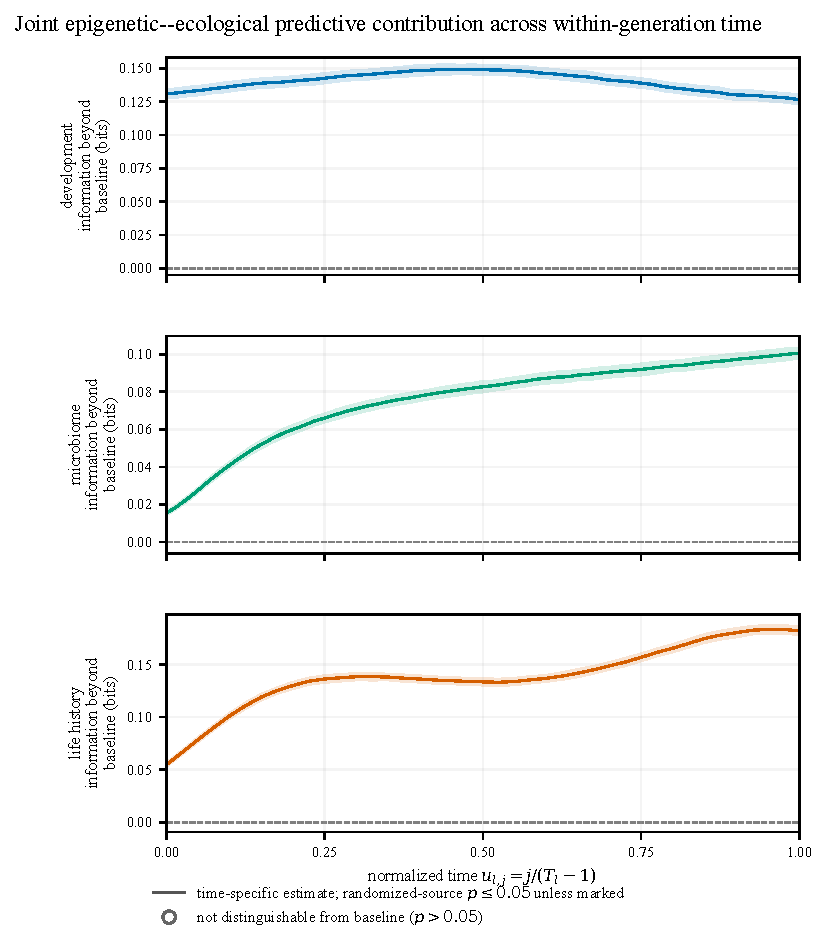
\includegraphics[width=0.58\textwidth]
{figures/figure08_joint_epigenetic_ecological_location.pdf}
\caption{Predictive contribution of the epigenetic-ecological configuration across normalized target time. Lines show information beyond baseline, bands show $95\%$ confidence intervals, and open markers indicate $p>0.05$.}
\label{fig:joint-location}
\end{figure}

To test whether the epigenetic-ecological configuration provides predictive information about the reconstruction of the focal variant $\nu=(0,0)$, we evaluated Equation~\ref{eq:joint-focal-information}:
\begin{equation}
I\left(
\mathbf{1}\left\{V_{d,\tau+1}=\nu\right\};
\mathbf{J}_{d,\tau}
\mid
\mathcal{X}^{\ELC\setminus
\{[l_{\mathrm{epigenetic}}],[l_{\mathrm{ecological}}]\},(k)}_{d,\tau}
\right).
\label{eq:joint-focal-information}
\end{equation}
The epigenetic-ecological configuration provided $0.0274$ bits about whether $\nu$ was reconstructed, with a $95\%$ confidence interval of $[0.0256,0.0292]$. The mean log-ratio for $\nu$ was $0.0634$ bits, with a $95\%$ confidence interval of $[0.0573,0.0696]$.

To test whether changing the epigenetic-ecological configuration increases the probability of $\nu=(0,0)$, we intervened on the two epigenetic and three ecological niche states at $t_l=0$ using $\boldsymbol{\theta}_x$. Later states were generated by the ELC dynamics. The intervention distribution is given by Equation~\ref{eq:joint-intervention-distribution}:
\begin{equation}
\begin{aligned}
&p_{\boldsymbol{\theta}_x}\left(
V_{d,\tau+1}
\mid
\mathcal{X}^{\ELC\setminus
\{[l_{\mathrm{epigenetic}}],[l_{\mathrm{ecological}}]\},(k)}_{d,\tau}
\right)
\\
&=
p\left(
V_{d,\tau+1}
\mid
\operatorname{do}\left[
\begin{pmatrix}
\mathbf{x}^{[l_{\mathrm{epigenetic}}]}_{d,t_l=0(\tau)}\\
\mathbf{x}^{[l_{\mathrm{ecological}}]}_{d,t_l=0(\tau)}
\end{pmatrix}
=
\begin{pmatrix}
\mathbf{x}^{[l_{\mathrm{epigenetic}}]}_{d,t_l=0(\tau)}\\
\mathbf{x}^{[l_{\mathrm{ecological}}]}_{d,t_l=0(\tau)}
\end{pmatrix}
+
\boldsymbol{\theta}_x
\right],
\mathcal{X}^{\ELC\setminus
\{[l_{\mathrm{epigenetic}}],[l_{\mathrm{ecological}}]\},(k)}_{d,\tau}
\right).
\end{aligned}
\label{eq:joint-intervention-distribution}
\end{equation}
At $\boldsymbol{\theta}_x=(-0.5,-0.5,-0.5,-0.5,-0.5)$, the probability of $\nu$ increased from $0.264$ to $0.590$. The increase was $0.326$, with a $95\%$ confidence interval of $[0.316,0.336]$. The local gradient at $\boldsymbol{\theta}_x=\mathbf{0}$ is given by Equation~\ref{eq:joint-local-gradient}:
\begin{equation}
\left.
\nabla_{\boldsymbol{\theta}_x}
p_{\boldsymbol{\theta}_x}\left(
V_{d,\tau+1}=\nu
\right)
\right|_{\boldsymbol{\theta}_x=\mathbf{0}}
=
\left(
-0.207,
0.0168,
-0.0265,
-0.290,
-0.0962
\right).
\label{eq:joint-local-gradient}
\end{equation}
The coordinates are ordered as
$(\theta_{\mathrm{reg}},
\theta_{\mathrm{stress}},
\theta_{\mathrm{soil}},
\theta_{\mathrm{resource}},
\theta_{\mathrm{microclimate}})$.
Causal specificity of the epigenetic-ecological configuration was evaluated using Equations~\ref{eq:fisher-context-final} and \ref{eq:fisher-average-final}, with $\mathcal{X}^{\ELC\setminus\{[l_{\mathrm{epigenetic}}],[l_{\mathrm{ecological}}]\},(k)}_{d,\tau}$ as the conditioning ELC history. The Fisher information matrix is given by Equation~\ref{eq:joint-fisher-matrix-final}:
\begin{equation}
\overline{\mathbf{F}}_{\mathrm{epi+eco}}(\mathbf{0})
=
\begin{pmatrix}
0.638 & -0.0639 & 0.0846 & 0.737 & 0.331 \\
-0.0639 & 0.0132 & -0.0122 & -0.0313 & -0.0448 \\
0.0846 & -0.0122 & 0.0156 & 0.0874 & 0.0491 \\
0.737 & -0.0313 & 0.0874 & 1.39 & 0.271 \\
0.331 & -0.0448 & 0.0491 & 0.271 & 0.208
\end{pmatrix}.
\label{eq:joint-fisher-matrix-final}
\end{equation}
All five diagonal entries are positive, indicating that changing any of the five intervention variables, the two epigenetic variables and three ecological niche variables, changes the probability distribution over the four phenotype states. The largest diagonal entry corresponds to $\theta_{\mathrm{resource}}$, indicating that the phenotype distribution was most sensitive to changes in resource availability.

Table~\ref{tab:complex-qualification} summarizes the complex unit of inheritance criteria:
\begin{table}[H]
\centering
\small
\setlength{\tabcolsep}{5pt}
\caption{Results for the complex-unit criteria.}
\label{tab:complex-qualification}
\begin{tabular}{@{}>{\raggedright\arraybackslash}p{0.35\textwidth}
>{\raggedright\arraybackslash}p{0.57\textwidth}@{}}
\toprule
Criterion & Result \\
\midrule
Predictive contribution
& $0.284$ bits beyond baseline, $p=0.002$ \\
Dependence on the ELC
& $0.0867$ bits beyond baseline, $p=0.002$ \\
Synergistic information about $\nu$
& $0.0110$ bits, $95\%$ CI $[0.00982,0.0122]$ \\
Predictive information about $\nu$
& $0.0274$ bits, $95\%$ CI $[0.0256,0.0292]$ \\
Increase in $p(\nu)$ after intervention
& $0.326$, $95\%$ CI $[0.316,0.336]$ \\
Causal specificity
& Positive Fisher diagonal entries for all five intervention coordinates \\
\bottomrule
\end{tabular}
\end{table}
Therefore, our results demonstrate that the epigenetic-ecological configuration satisfied the criteria for a complex unit of inheritance with respect to $\nu=(0,0)$.

\section{Recovery of Dependency Structure}
We tested whether the estimator recovered the cross-level couplings specified by the transition equations. For each source and target level, we estimated the information transferred from the source in generation $\tau$ to the target in generation $\tau+1$ and compared this estimate with the corresponding permutation baseline. A dependency was counted as recovered when the estimated information exceeded the permutation baseline at $p\leq0.01$.

Figure~\ref{fig:model-check-networks} compares the specified and detected couplings:
\begin{figure}[H]
\centering
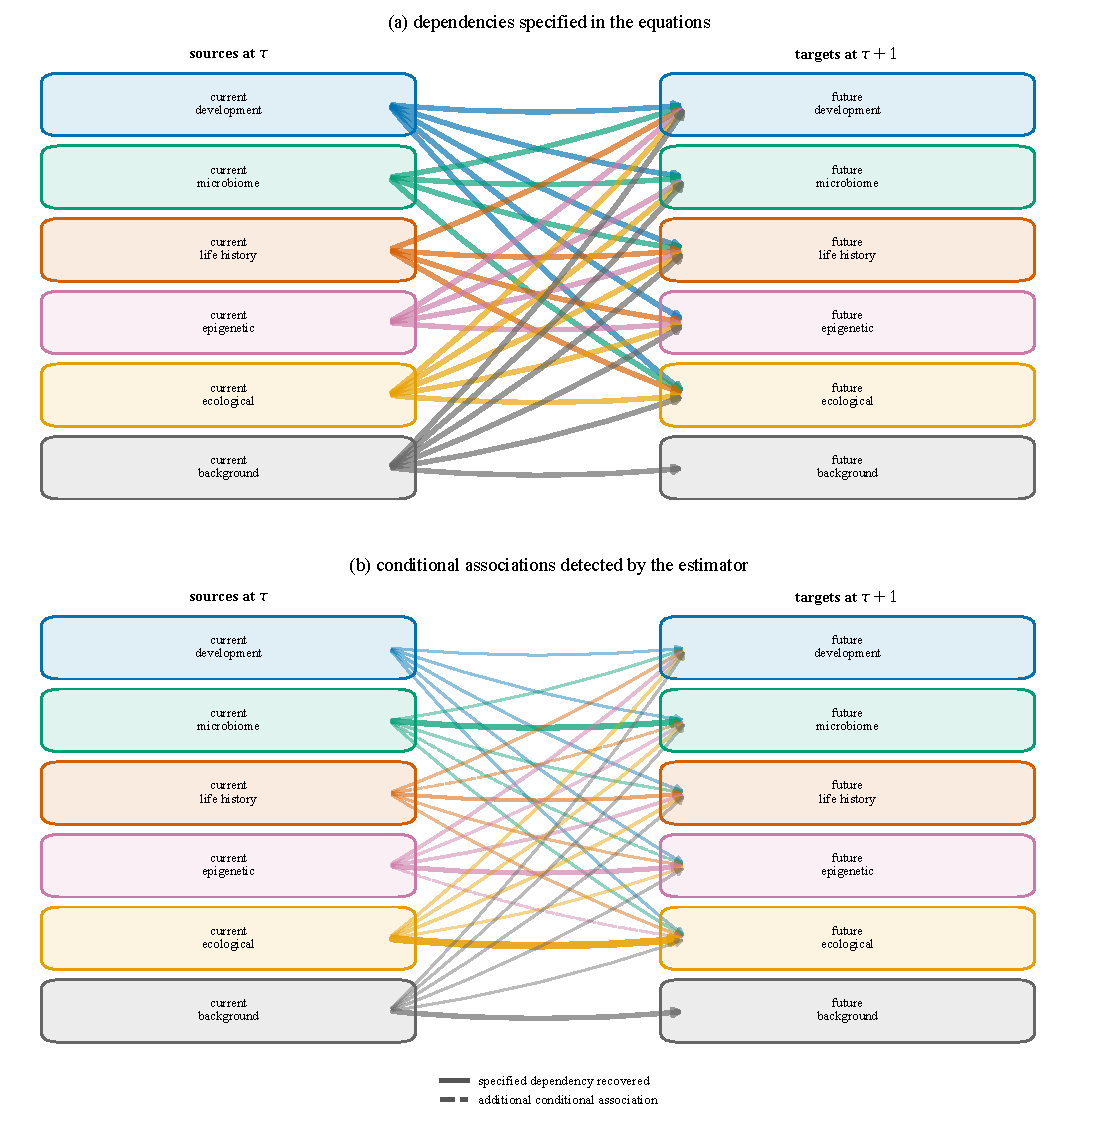
\includegraphics[width=0.96\textwidth]
{figures/figure03_coupling_networks.pdf}
\caption{True and detected couplings. Panel (a) shows the $28$ true dependencies specified by the transition equations. Panel (b) shows the dependencies detected at $p\leq0.01$. All specified dependencies were recovered. Dashed links show three additional associations.}
\label{fig:model-check-networks}
\end{figure}

Figure~\ref{fig:model-check-matrix} reports the corresponding information estimates:
\begin{figure}[H]
\centering
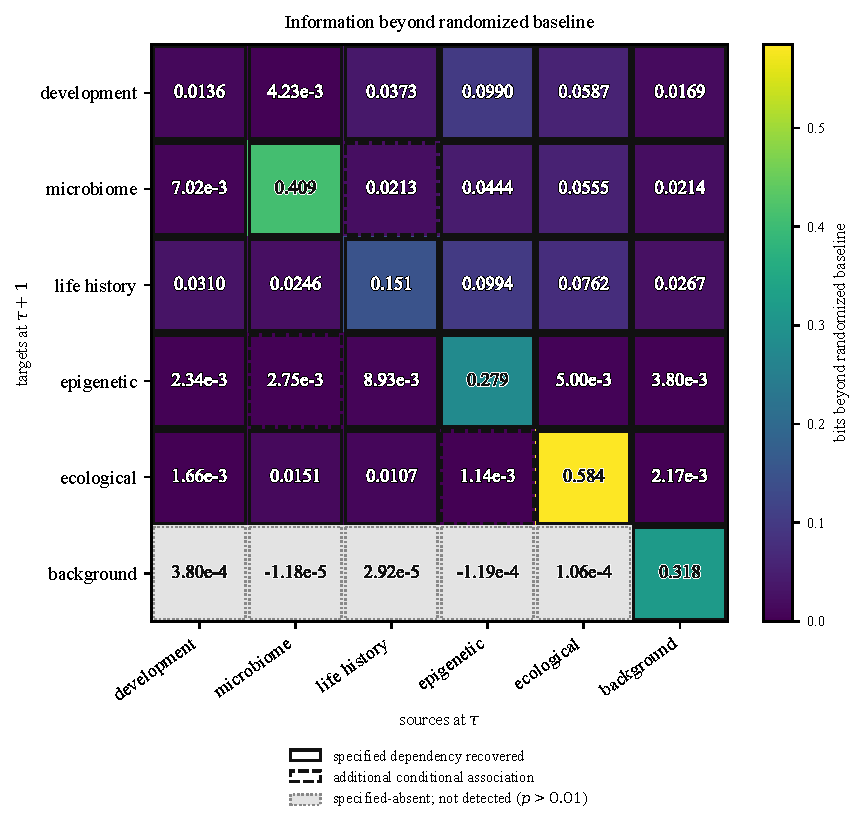
\includegraphics[width=0.86\textwidth]
{figures/figure04_coupling_information_matrix.pdf}
\caption{Information beyond the permutation baseline for each source-target pair. Rows are target levels in generation $\tau+1$, and columns are source levels in generation $\tau$. Solid outlines mark specified dependencies, dashed outlines mark additional associations, and dotted outlines mark comparisons without specified couplings. Gray cells indicate $p>0.01$.}
\label{fig:model-check-matrix}
\end{figure}
All $28$ specified dependencies were recovered, and none of the five comparisons without specified couplings were detected. Three additional associations were detected: life history to microbiome $(0.0213$ bits$)$, microbiome to epigenetic $(0.00275$ bits$)$, and epigenetic to ecology $(0.00114$ bits$)$. These associations may result from indirect paths through the ELC.

\section{Reproducibility}
Table~\ref{tab:simulation-design} reports the simulation and analysis settings.
\begin{table}[H]
\centering
\small
\setlength{\tabcolsep}{3pt}
\caption{Simulation and analysis settings.}
\label{tab:simulation-design}
\begin{tabular}{@{}>{\raggedright\arraybackslash}p{0.30\textwidth}
>{\raggedright\arraybackslash}p{0.62\textwidth}@{}}
\toprule
Quantity & Value \\
\midrule
Primary simulation seeds
& 254989981, 265358979, 276563425, 287271829 \\
Additional ELC simulation seeds
& 298463771, 309016999, 320377241, 331662479 \\
Lineages per seed
& 1000 \\
Generations per lineage
& 32 \\
Burn-in generations
& 8 \\
Generations analyzed
& 8-30 \\
History order
& $k=2$ \\
Bootstrap replicates
& 500 for transfer entropy and interventions; 300 for PID \\
Permutation replicates
& 500 \\
Intervention contexts
& 1000 \\
Simulations per context and intervention
& 1000 \\
Phenotype thresholds
& $\theta_M=0.60$, $u_{\mathrm{early}}=0.60$, $\theta_G=0.65$ \\
\bottomrule
\end{tabular}
\end{table}

\appendix
\section{Complete Equations and Parameter Values}
This appendix lists the equations and parameter values used in the simulation. Time during each generation is normalized to $u\in[0,1]$. Each level is updated on its own time grid using the most recent states of the other levels. For level $l$, $n_l$ is the number of updates from $u=0$ to $u=1$, and $\Delta u=1/n_l$ is the time between updates. The developmental gene regulatory network level uses $n_l=280$; the microbiome level uses $n_l=360$; the life history level uses $n_l=200$; and the epigenetic level, ecological level, and background process each use $n_l=160$. A scalar Brownian increment for one update is $dW=\sqrt{\Delta u}\,\eta$, where $\eta\sim\mathcal{N}(0,1)$. For each generation, level $l$ has a time series of length $T_l$. The developmental level uses $(T_l,m_l)=(57,8)$; the microbiome level uses $(T_l,m_l)=(61,10)$; the life history level uses $(T_l,m_l)=(41,5)$; and the epigenetic level, ecological level, and background process each use $(T_l,m_l)=(33,5)$. The logistic function used below is $\sigma(z)=1/(1+\exp(-z))$. Equation~\ref{eq:appendix-phase-functions} defines three functions that depend on time $u$, lineage $d$, and generation $\tau$. The value $\psi_d$ assigns lineage $d$ one of $37$ phase offsets. The expression $(d+1)\bmod 37$ takes a value from $0$ to $36$:
\begin{equation}
\begin{aligned}
\psi_d
&=
2\pi\frac{(d+1)\bmod 37}{37},
\\
\phi_{\mathrm{dev}}(u,d,\tau)
&=
\sin(2\pi u+\psi_d+0.41\tau),
\\
\phi_{\mathrm{micro}}(u,d,\tau)
&=
\cos(2\pi u-0.25\psi_d+0.29\tau),
\\
\phi_{\mathrm{slow}}(u,d,\tau)
&=
\sin(\pi u+0.17\tau+0.5\psi_d).
\end{aligned}
\label{eq:appendix-phase-functions}
\end{equation}

\subsection{Developmental GRN Functions and Parameters}
The developmental GRN matrix is given by Equation~\ref{eq:appendix-dev-matrix}:
\begin{equation}
A_{\mathrm{dev}}
=
\begin{pmatrix}
-0.80 & 0.70 & 0.00 & -0.40 & 0.60\\
-0.50 & -0.90 & 0.80 & 0.00 & -0.20\\
0.30 & -0.60 & -0.70 & 0.90 & 0.00\\
0.00 & 0.40 & -0.50 & -1.00 & 0.60\\
0.70 & 0.00 & 0.30 & -0.60 & -0.80
\end{pmatrix}.
\label{eq:appendix-dev-matrix}
\end{equation}
The developmental cross-level interaction term is given by Equation~\ref{eq:appendix-dev-cross-level}:
\begin{equation}
\begin{aligned}
&\mathbf{C}_{d}^{[l_{\mathrm{development}}]}
\left\{
\mathbf{x}_{d,t_l(\tau)}^{[l']}
\right\}_{l'\neq l_{\mathrm{development}}}
\\
&=
\begin{pmatrix}
0.952\!\left[\sigma\!\left(x^{[l_{\mathrm{epigenetic}}]}_{d,\mathrm{reg},t_l(\tau)}\right)-0.5\right]\\
0.18\log\!\left(1+x^{[l_{\mathrm{microbiome}}]}_{d,1,t_l(\tau)}\right)
+0.22x^{[l_{\mathrm{ecological}}]}_{d,2,t_l(\tau)}\\
0.16\log\!\left(1+x^{[l_{\mathrm{microbiome}}]}_{d,4,t_l(\tau)}\right)
+0.784\!\left[\sigma\!\left(x^{[l_{\mathrm{epigenetic}}]}_{d,\mathrm{stress},t_l(\tau)}\right)-0.5\right]\\
0.15x^{[l_{\mathrm{life\text{-}history}}]}_{d,\mathrm{mat},t_l(\tau)}\\
0.18x^{[l_{\mathrm{ecological}}]}_{d,3,t_l(\tau)}
+0.12x^{[l_{\mathrm{life\text{-}history}}]}_{d,\mathrm{repr},t_l(\tau)}
\end{pmatrix}.
\end{aligned}
\label{eq:appendix-dev-cross-level}
\end{equation}
The external developmental input is given by Equation~\ref{eq:appendix-dev-external}:
\begin{equation}
\mathbf{u}^{[l_{\mathrm{development}}]}_{d,t_l(\tau)}
=
\begin{pmatrix}
0.15\phi_{\mathrm{dev}}(u,d,\tau)\\
0.10x^{[l_{\mathrm{background}}]}_{d,1,t_l(\tau)}
+0.20\phi_{\mathrm{slow}}(u,d,\tau)\\
0.12x^{[l_{\mathrm{background}}]}_{d,2,t_l(\tau)}
-0.12\phi_{\mathrm{micro}}(u,d,\tau)\\
0.18\sin(\pi u)\\
0.16\cos(\pi u)
\end{pmatrix}.
\label{eq:appendix-dev-external}
\end{equation}

\subsection{Microbiome Functions and Parameters}
The microbiome interaction matrix is given by Equation~\ref{eq:appendix-micro-matrix}:
\begin{equation}
A_{\mathrm{micro}}
=
\begin{pmatrix}
-0.74 & 0.14 & -0.08 & -0.12 & 0.18\\
0.10 & -0.68 & 0.12 & -0.08 & 0.08\\
-0.08 & 0.10 & -0.70 & 0.15 & -0.06\\
-0.16 & -0.10 & 0.12 & -0.64 & 0.08\\
0.14 & 0.12 & -0.06 & 0.10 & -0.66
\end{pmatrix}.
\label{eq:appendix-micro-matrix}
\end{equation}
The functions $r_{d,i,t_{l_{\mathrm{microbiome}}}(\tau)}$ specify the growth rates of the five microbiome guilds. The five growth rates are given by Equation~\ref{eq:appendix-micro-growth}:
\begin{equation}
\begin{aligned}
r_{d,1,t_{l_{\mathrm{microbiome}}}(\tau)}
&=0.50
+5.40\tanh\!\left(
x^{[l_{\mathrm{development}}]}_{d,2,t_{l_{\mathrm{development}}}(\tau)}
\right)\\
&\quad
+0.25\left[
\sigma\!\left(
x^{[l_{\mathrm{epigenetic}}]}_{d,\mathrm{reg},t_{l_{\mathrm{epigenetic}}}(\tau)}
\right)-0.5
\right]\\
&\quad
+0.20x^{[l_{\mathrm{ecological}}]}_{d,2,t_{l_{\mathrm{ecological}}}(\tau)}
+0.08x^{[l_{\mathrm{background}}]}_{d,1,t_{l_{\mathrm{background}}}(\tau)}
+0.10\phi_{\mathrm{micro}}(u,d,\tau),\\
r_{d,2,t_{l_{\mathrm{microbiome}}}(\tau)}
&=0.38
+0.18x^{[l_{\mathrm{ecological}}]}_{d,1,t_{l_{\mathrm{ecological}}}(\tau)}
+0.08\phi_{\mathrm{slow}}(u,d,\tau),\\
r_{d,3,t_{l_{\mathrm{microbiome}}}(\tau)}
&=0.34
-0.16x^{[l_{\mathrm{ecological}}]}_{d,3,t_{l_{\mathrm{ecological}}}(\tau)}
+2.40\tanh\!\left(
x^{[l_{\mathrm{development}}]}_{d,3,t_{l_{\mathrm{development}}}(\tau)}
\right),\\
r_{d,4,t_{l_{\mathrm{microbiome}}}(\tau)}
&=0.30
+4.80\tanh\!\left(
x^{[l_{\mathrm{development}}]}_{d,3,t_{l_{\mathrm{development}}}(\tau)}
\right)\\
&\quad
+0.30\left[
\sigma\!\left(
x^{[l_{\mathrm{epigenetic}}]}_{d,\mathrm{stress},t_{l_{\mathrm{epigenetic}}}(\tau)}
\right)-0.5
\right]\\
&\quad
+0.10x^{[l_{\mathrm{background}}]}_{d,2,t_{l_{\mathrm{background}}}(\tau)}
-0.10\phi_{\mathrm{micro}}(u,d,\tau),\\
r_{d,5,t_{l_{\mathrm{microbiome}}}(\tau)}
&=0.40
+0.10x^{[l_{\mathrm{microbiome}}]}_{d,1,t_{l_{\mathrm{microbiome}}}(\tau)}
+0.07x^{[l_{\mathrm{ecological}}]}_{d,1,t_{l_{\mathrm{ecological}}}(\tau)}.
\end{aligned}
\label{eq:appendix-micro-growth}
\end{equation}

\subsection{Life History Functions}
The functions used in Equation~\ref{eq:life-equation} are given by Equation~\ref{eq:appendix-life-functions}. The developmental, microbiome, epigenetic, and ecological terms instantiate $\mathbf{C}^{[l_{\mathrm{life\text{-}history}}]}_d$. The functions also include the current life history state, the background process, and time $u$:
\begin{equation}
\begin{aligned}
\eta_{d,t_{l_{\mathrm{life\text{-}history}}}(\tau)}
&=0.25
-0.10\tanh\!\left(
x^{[l_{\mathrm{development}}]}_{d,4,t_{l_{\mathrm{development}}}(\tau)}
\right)\\
&\quad
-0.08\log\!\left(
1+x^{[l_{\mathrm{microbiome}}]}_{d,1,t_{l_{\mathrm{microbiome}}}(\tau)}
\right)\\
&\quad
-0.315\left[
\sigma\!\left(
x^{[l_{\mathrm{epigenetic}}]}_{d,\mathrm{reg},t_{l_{\mathrm{epigenetic}}}(\tau)}
\right)-0.5
\right]\\
&\quad
+0.06x^{[l_{\mathrm{background}}]}_{d,2,t_{l_{\mathrm{background}}}(\tau)},\\
\omega_{\mathrm{mat},d,t_{l_{\mathrm{life\text{-}history}}}(\tau)}
&=
\sigma\!\left(
8\left[
u-\eta_{d,t_{l_{\mathrm{life\text{-}history}}}(\tau)}
\right]
\right),\\
\omega_{\mathrm{late},d,t_{l_{\mathrm{life\text{-}history}}}(\tau)}
&=
\sigma\!\left(10(u-0.72)\right),\\
\alpha_{d,t_{l_{\mathrm{life\text{-}history}}}(\tau)}
&=
\sigma\!\left(
9\left[
u-0.55
+0.06x^{[l_{\mathrm{background}}]}_{d,2,t_{l_{\mathrm{background}}}(\tau)}
-0.05x^{[l_{\mathrm{life\text{-}history}}]}_{d,\mathrm{grow},t_{l_{\mathrm{life\text{-}history}}}(\tau)}
\right]
\right),\\
U_{\mathrm{mat},d,t_{l_{\mathrm{life\text{-}history}}}(\tau)}
&=-0.92
+2.22\omega_{\mathrm{mat},d,t_{l_{\mathrm{life\text{-}history}}}(\tau)}\\
&\quad
+0.42\tanh\!\left(
x^{[l_{\mathrm{development}}]}_{d,4,t_{l_{\mathrm{development}}}(\tau)}
\right)\\
&\quad
+0.18\log\!\left(
1+x^{[l_{\mathrm{microbiome}}]}_{d,1,t_{l_{\mathrm{microbiome}}}(\tau)}
\right)\\
&\quad
+0.750\left[
\sigma\!\left(
x^{[l_{\mathrm{epigenetic}}]}_{d,\mathrm{reg},t_{l_{\mathrm{epigenetic}}}(\tau)}
\right)-0.5
\right]\\
&\quad
+0.1312x^{[l_{\mathrm{ecological}}]}_{d,3,t_{l_{\mathrm{ecological}}}(\tau)}
-0.16x^{[l_{\mathrm{background}}]}_{d,2,t_{l_{\mathrm{background}}}(\tau)}
+0.20\phi_{\mathrm{slow}}(u,d,\tau),\\
U_{\mathrm{grow},d,t_{l_{\mathrm{life\text{-}history}}}(\tau)}
&=-0.05
+0.66\tanh\!\left(
x^{[l_{\mathrm{development}}]}_{d,2,t_{l_{\mathrm{development}}}(\tau)}
\right)\\
&\quad
+0.36\log\!\left(
1+x^{[l_{\mathrm{microbiome}}]}_{d,1,t_{l_{\mathrm{microbiome}}}(\tau)}
+0.6x^{[l_{\mathrm{microbiome}}]}_{d,2,t_{l_{\mathrm{microbiome}}}(\tau)}
\right)\\
&\quad
+1.68\left[
\sigma\!\left(
x^{[l_{\mathrm{epigenetic}}]}_{d,\mathrm{reg},t_{l_{\mathrm{epigenetic}}}(\tau)}
\right)-0.5
\right]\\
&\quad
+0.2788x^{[l_{\mathrm{ecological}}]}_{d,2,t_{l_{\mathrm{ecological}}}(\tau)}
+0.10x^{[l_{\mathrm{background}}]}_{d,1,t_{l_{\mathrm{background}}}(\tau)}\\
&\quad
-0.24x^{[l_{\mathrm{life\text{-}history}}]}_{d,\mathrm{repr},t_{l_{\mathrm{life\text{-}history}}}(\tau)}
+0.42\sin(\pi u)\\
&\quad
-0.28\omega_{\mathrm{late},d,t_{l_{\mathrm{life\text{-}history}}}(\tau)}
+0.16\phi_{\mathrm{micro}}(u,d,\tau),\\
U_{\mathrm{repr},d,t_{l_{\mathrm{life\text{-}history}}}(\tau)}
&=-1.26
+1.18x^{[l_{\mathrm{life\text{-}history}}]}_{d,\mathrm{mat},t_{l_{\mathrm{life\text{-}history}}}(\tau)}
+0.62x^{[l_{\mathrm{life\text{-}history}}]}_{d,\mathrm{grow},t_{l_{\mathrm{life\text{-}history}}}(\tau)}\\
&\quad
+0.30\alpha_{d,t_{l_{\mathrm{life\text{-}history}}}(\tau)}
+0.24\tanh\!\left(
x^{[l_{\mathrm{development}}]}_{d,5,t_{l_{\mathrm{development}}}(\tau)}
\right)\\
&\quad
+0.770\left[
\sigma\!\left(
x^{[l_{\mathrm{epigenetic}}]}_{d,\mathrm{stress},t_{l_{\mathrm{epigenetic}}}(\tau)}
\right)-0.5
\right]\\
&\quad
+0.1804x^{[l_{\mathrm{ecological}}]}_{d,1,t_{l_{\mathrm{ecological}}}(\tau)}
-0.16x^{[l_{\mathrm{background}}]}_{d,2,t_{l_{\mathrm{background}}}(\tau)}\\
&\quad
+0.18\phi_{\mathrm{dev}}(u,d,\tau)\\
&\quad
-0.16x^{[l_{\mathrm{life\text{-}history}}]}_{d,\mathrm{grow},t_{l_{\mathrm{life\text{-}history}}}(\tau)}
\omega_{\mathrm{late},d,t_{l_{\mathrm{life\text{-}history}}}(\tau)},\\
\mathbf{U}_{d,t_{l_{\mathrm{life\text{-}history}}}(\tau)}
&=
\left(
U_{\mathrm{mat},d,t_{l_{\mathrm{life\text{-}history}}}(\tau)},
U_{\mathrm{grow},d,t_{l_{\mathrm{life\text{-}history}}}(\tau)},
U_{\mathrm{repr},d,t_{l_{\mathrm{life\text{-}history}}}(\tau)}
\right)^{\top}.
\end{aligned}
\label{eq:appendix-life-functions}
\end{equation}

\subsection{Epigenetic Functions}
The logistic function is applied within the Hill functions to bound the values between $0$ and $1$. The functions are given by Equation~\ref{eq:appendix-hill}:
\begin{equation}
\begin{aligned}
H_{\mathrm{reg}}\!\left(
x^{[l_{\mathrm{epigenetic}}]}_{d,\mathrm{reg},t_l(\tau)}
\right)
&=
\frac{
\sigma\!\left(
x^{[l_{\mathrm{epigenetic}}]}_{d,\mathrm{reg},t_l(\tau)}
\right)^3
}{
0.52^3+
\sigma\!\left(
x^{[l_{\mathrm{epigenetic}}]}_{d,\mathrm{reg},t_l(\tau)}
\right)^3
},\\
H_{\mathrm{stress}}\!\left(
x^{[l_{\mathrm{epigenetic}}]}_{d,\mathrm{stress},t_l(\tau)}
\right)
&=
\frac{
\sigma\!\left(
x^{[l_{\mathrm{epigenetic}}]}_{d,\mathrm{stress},t_l(\tau)}
\right)^3
}{
0.50^3+
\sigma\!\left(
x^{[l_{\mathrm{epigenetic}}]}_{d,\mathrm{stress},t_l(\tau)}
\right)^3
}.
\end{aligned}
\label{eq:appendix-hill}
\end{equation}

The epigenetic input functions are given by Equation~\ref{eq:appendix-epi-g}:
\begin{equation}
\begin{aligned}
G_{\mathrm{reg},d,t_l(\tau)}
&=
0.38\left[
2H_{\mathrm{reg}}\!\left(
x^{[l_{\mathrm{epigenetic}}]}_{d,\mathrm{reg},t_l(\tau)}
\right)-1
\right]
-
0.26\left[
2H_{\mathrm{stress}}\!\left(
x^{[l_{\mathrm{epigenetic}}]}_{d,\mathrm{stress},t_l(\tau)}
\right)-1
\right]\\
&\quad+
0.32\tanh\!\left(
x^{[l_{\mathrm{development}}]}_{d,1,t_l(\tau)}
\right)
+
0.22x^{[l_{\mathrm{life\text{-}history}}]}_{d,\mathrm{grow},t_l(\tau)}
+
0.20x^{[l_{\mathrm{ecological}}]}_{d,2,t_l(\tau)}\\
&\quad-
0.14x^{[l_{\mathrm{background}}]}_{d,2,t_l(\tau)}
+
0.20\phi_{\mathrm{slow}}(u,d,\tau),\\
G_{\mathrm{stress},d,t_l(\tau)}
&=
0.36\left[
2H_{\mathrm{stress}}\!\left(
x^{[l_{\mathrm{epigenetic}}]}_{d,\mathrm{stress},t_l(\tau)}
\right)-1
\right]
-
0.24\left[
2H_{\mathrm{reg}}\!\left(
x^{[l_{\mathrm{epigenetic}}]}_{d,\mathrm{reg},t_l(\tau)}
\right)-1
\right]\\
&\quad+
0.30\tanh\!\left(
x^{[l_{\mathrm{development}}]}_{d,3,t_l(\tau)}
\right)
+
0.28x^{[l_{\mathrm{life\text{-}history}}]}_{d,\mathrm{repr},t_l(\tau)}
-
0.16x^{[l_{\mathrm{ecological}}]}_{d,3,t_l(\tau)}\\
&\quad+
0.22x^{[l_{\mathrm{background}}]}_{d,2,t_l(\tau)}
+
0.18\phi_{\mathrm{micro}}(u,d,\tau).
\end{aligned}
\label{eq:appendix-epi-g}
\end{equation}


\subsection{Ecological Niche Functions}
The ecological functions in Equation~\ref{eq:ecological-equation} are given by Equation~\ref{eq:appendix-eco-rm}:
\begin{equation}
\begin{aligned}
R_{1,d,t_{l_{\mathrm{ecological}}}(\tau)}
&=
-0.22x^{[l_{\mathrm{ecological}}]}_{d,1,t_{l_{\mathrm{ecological}}}(\tau)}
+0.06\tanh\!\left(
x^{[l_{\mathrm{ecological}}]}_{d,2,t_{l_{\mathrm{ecological}}}(\tau)}
\right)
-0.04\left(
x^{[l_{\mathrm{ecological}}]}_{d,1,t_{l_{\mathrm{ecological}}}(\tau)}
\right)^3,\\
R_{2,d,t_{l_{\mathrm{ecological}}}(\tau)}
&=
-0.20x^{[l_{\mathrm{ecological}}]}_{d,2,t_{l_{\mathrm{ecological}}}(\tau)}
+0.05\tanh\!\left(
x^{[l_{\mathrm{ecological}}]}_{d,1,t_{l_{\mathrm{ecological}}}(\tau)}
\right)\\
&\quad+
0.04\tanh\!\left(
x^{[l_{\mathrm{ecological}}]}_{d,3,t_{l_{\mathrm{ecological}}}(\tau)}
\right)
-0.04\left(
x^{[l_{\mathrm{ecological}}]}_{d,2,t_{l_{\mathrm{ecological}}}(\tau)}
\right)^3,\\
R_{3,d,t_{l_{\mathrm{ecological}}}(\tau)}
&=
-0.18x^{[l_{\mathrm{ecological}}]}_{d,3,t_{l_{\mathrm{ecological}}}(\tau)}
+0.06\tanh\!\left(
x^{[l_{\mathrm{ecological}}]}_{d,2,t_{l_{\mathrm{ecological}}}(\tau)}
\right)
-0.04\left(
x^{[l_{\mathrm{ecological}}]}_{d,3,t_{l_{\mathrm{ecological}}}(\tau)}
\right)^3,\\
M_{1,d,t_{l_{\mathrm{ecological}}}(\tau)}
&=
0.30\log\!\left(
1+x^{[l_{\mathrm{microbiome}}]}_{d,1,t_{l_{\mathrm{microbiome}}}(\tau)}
\right)
+0.24x^{[l_{\mathrm{life\text{-}history}}]}_{d,\mathrm{repr},t_{l_{\mathrm{life\text{-}history}}}(\tau)}
-0.06x^{[l_{\mathrm{background}}]}_{d,2,t_{l_{\mathrm{background}}}(\tau)},\\
M_{2,d,t_{l_{\mathrm{ecological}}}(\tau)}
&=
0.28\tanh\!\left(
x^{[l_{\mathrm{development}}]}_{d,2,t_{l_{\mathrm{development}}}(\tau)}
\right)
+0.32x^{[l_{\mathrm{life\text{-}history}}]}_{d,\mathrm{repr},t_{l_{\mathrm{life\text{-}history}}}(\tau)}\\
&\quad+
0.12\log\!\left(
1+x^{[l_{\mathrm{microbiome}}]}_{d,1,t_{l_{\mathrm{microbiome}}}(\tau)}
\right)
+0.06\phi_{\mathrm{slow}}(u,d,\tau),\\
M_{3,d,t_{l_{\mathrm{ecological}}}(\tau)}
&=
0.22x^{[l_{\mathrm{life\text{-}history}}]}_{d,\mathrm{mat},t_{l_{\mathrm{life\text{-}history}}}(\tau)}
+0.20\log\!\left(
1+x^{[l_{\mathrm{microbiome}}]}_{d,5,t_{l_{\mathrm{microbiome}}}(\tau)}
\right)\\
&\quad-
0.08x^{[l_{\mathrm{background}}]}_{d,2,t_{l_{\mathrm{background}}}(\tau)}
+0.08\phi_{\mathrm{dev}}(u,d,\tau),\\
\mathbf{R}^{[l_{\mathrm{ecological}}]}_{d,t_{l_{\mathrm{ecological}}}(\tau)}
&=
\left(
R_{1,d,t_{l_{\mathrm{ecological}}}(\tau)},
R_{2,d,t_{l_{\mathrm{ecological}}}(\tau)},
R_{3,d,t_{l_{\mathrm{ecological}}}(\tau)}
\right)^\top,\\
\mathbf{M}^{[l_{\mathrm{ecological}}]}_{d,t_{l_{\mathrm{ecological}}}(\tau)}
&=
\left(
M_{1,d,t_{l_{\mathrm{ecological}}}(\tau)},
M_{2,d,t_{l_{\mathrm{ecological}}}(\tau)},
M_{3,d,t_{l_{\mathrm{ecological}}}(\tau)}
\right)^\top.
\end{aligned}
\label{eq:appendix-eco-rm}
\end{equation}

\subsection{Noise Amplitudes}
The noise amplitudes are listed in the component order of each state vector in Equation~\ref{eq:appendix-noise}:
\begin{equation}
\begin{aligned}
\boldsymbol{\sigma}_{\mathrm{dev}}
&=(0.12,0.11,0.13,0.11,0.12),\\
\boldsymbol{\sigma}_{\mathrm{micro}}
&=(0.16,0.15,0.16,0.17,0.15),\\
\boldsymbol{\sigma}_{\mathrm{life}}
&=(0.14,0.13,0.15),\\
\boldsymbol{\sigma}_{\mathrm{epi}}
&=(0.24,0.24),\\
\boldsymbol{\sigma}_{\mathrm{eco}}
&=(0.13,0.13,0.12),\\
\boldsymbol{\sigma}_{\mathrm{background}}
&=(0.16,0.16).
\end{aligned}
\label{eq:appendix-noise}
\end{equation}

The reproductive transition occurs at $u_R=0.75$. For level $l$, the last time point at or before $u_R$ is given by Equation~\ref{eq:appendix-reproductive-state}:
\begin{equation}
j_l^R
=
\max\left\{
j:t_{l,j}\leq u_R
\right\}.
\label{eq:appendix-reproductive-state}
\end{equation}
The state used at the reproductive transition is $\mathbf{x}^{[l]}_{d,t_{l,j_l^R}(\tau)}$. These states determine the states at $t_l=0$ in generation $\tau+1$.

The background state at $t_l=0$ in generation $\tau+1$ is given by Equation~\ref{eq:appendix-background-start}:
\begin{equation}
\mathbf{x}^{[l_{\mathrm{background}}]}_{d,t_l=0(\tau+1)}
=
\begin{pmatrix}
0.65&0\\
0&0.60
\end{pmatrix}
\mathbf{x}^{[l_{\mathrm{background}}]}_{d,t_{l_{\mathrm{background}},j_{\mathrm{background}}^R}(\tau)}
+
\boldsymbol{\epsilon}^{[l_{\mathrm{background}}]}_{d,\tau}.
\label{eq:appendix-background-start}
\end{equation}
Here, $\boldsymbol{\epsilon}^{[l_{\mathrm{background}}]}_{d,\tau}\sim\mathcal{N}(\mathbf{0},0.20^2I_2)$.

The epigenetic state of $d$ at $t_l=0$ in generation $\tau+1$ is given by Equation~\ref{eq:appendix-epigenetic-start}:
\begin{equation}
\mathbf{x}^{[l_{\mathrm{epigenetic}}]}_{d,t_l=0(\tau+1)}
=
\begin{pmatrix}
0.72x^{[l_{\mathrm{epigenetic}}]}_{d,\mathrm{reg},t_{l_{\mathrm{epigenetic}},j_{\mathrm{epigenetic}}^R}(\tau)}\\
0.70x^{[l_{\mathrm{epigenetic}}]}_{d,\mathrm{stress},t_{l_{\mathrm{epigenetic}},j_{\mathrm{epigenetic}}^R}(\tau)}
\end{pmatrix}
+
\boldsymbol{\epsilon}^{[l_{\mathrm{epigenetic}}]}_{d,\tau}.
\label{eq:appendix-epigenetic-start}
\end{equation}
Here, $\boldsymbol{\epsilon}^{[l_{\mathrm{epigenetic}}]}_{d,\tau}\sim\mathcal{N}(\mathbf{0},0.16^2I_2)$.

The ecological state at $t_l=0$ in generation $\tau+1$ is given by Equation~\ref{eq:appendix-ecological-start}:
\begin{equation}
\begin{aligned}
x^{[l_{\mathrm{ecological}}]}_{d,1,t_l=0(\tau+1)}
&=0.64x^{[l_{\mathrm{ecological}}]}_{d,1,t_{l_{\mathrm{ecological}},j_{\mathrm{ecological}}^R}(\tau)}
+0.12x^{[l_{\mathrm{ecological}}]}_{d,2,t_{l_{\mathrm{ecological}},j_{\mathrm{ecological}}^R}(\tau)}\\
&\quad
+0.18\log\!\left(
1+x^{[l_{\mathrm{microbiome}}]}_{d,1,t_{l_{\mathrm{microbiome}},j_{\mathrm{microbiome}}^R}(\tau)}
\right)\\
&\quad
+0.18x^{[l_{\mathrm{life\text{-}history}}]}_{d,\mathrm{repr},t_{l_{\mathrm{life\text{-}history}},j_{\mathrm{life\text{-}history}}^R}(\tau)}
+\epsilon^{[l_{\mathrm{ecological}}]}_{d,1,\tau},\\
x^{[l_{\mathrm{ecological}}]}_{d,2,t_l=0(\tau+1)}
&=0.60x^{[l_{\mathrm{ecological}}]}_{d,2,t_{l_{\mathrm{ecological}},j_{\mathrm{ecological}}^R}(\tau)}
+0.10x^{[l_{\mathrm{ecological}}]}_{d,3,t_{l_{\mathrm{ecological}},j_{\mathrm{ecological}}^R}(\tau)}\\
&\quad
+0.18x^{[l_{\mathrm{life\text{-}history}}]}_{d,\mathrm{repr},t_{l_{\mathrm{life\text{-}history}},j_{\mathrm{life\text{-}history}}^R}(\tau)}\\
&\quad
+0.10\tanh\!\left(
x^{[l_{\mathrm{development}}]}_{d,2,t_{l_{\mathrm{development}},j_{\mathrm{development}}^R}(\tau)}
\right)
+\epsilon^{[l_{\mathrm{ecological}}]}_{d,2,\tau},\\
x^{[l_{\mathrm{ecological}}]}_{d,3,t_l=0(\tau+1)}
&=0.62x^{[l_{\mathrm{ecological}}]}_{d,3,t_{l_{\mathrm{ecological}},j_{\mathrm{ecological}}^R}(\tau)}
+0.14x^{[l_{\mathrm{ecological}}]}_{d,1,t_{l_{\mathrm{ecological}},j_{\mathrm{ecological}}^R}(\tau)}\\
&\quad
+0.12x^{[l_{\mathrm{life\text{-}history}}]}_{d,\mathrm{mat},t_{l_{\mathrm{life\text{-}history}},j_{\mathrm{life\text{-}history}}^R}(\tau)}\\
&\quad
+0.10\log\!\left(
1+x^{[l_{\mathrm{microbiome}}]}_{d,5,t_{l_{\mathrm{microbiome}},j_{\mathrm{microbiome}}^R}(\tau)}
\right)
+\epsilon^{[l_{\mathrm{ecological}}]}_{d,3,\tau}.
\end{aligned}
\label{eq:appendix-ecological-start}
\end{equation}
Here, $\boldsymbol{\epsilon}^{[l_{\mathrm{ecological}}]}_{d,\tau}\sim\mathcal{N}(\mathbf{0},0.16^2I_3)$.

The developmental GRN state at $t_l=0$ in generation $\tau+1$ is given by Equation~\ref{eq:appendix-development-start}:
\begin{equation}
\begin{aligned}
x^{[l_{\mathrm{development}}]}_{d,1,t_l=0(\tau+1)}
&=1.02\!\left[
\sigma\!\left(x^{[l_{\mathrm{epigenetic}}]}_{d,\mathrm{reg},t_l=0(\tau+1)}\right)-0.5
\right]
+0.10x^{[l_{\mathrm{ecological}}]}_{d,2,t_l=0(\tau+1)}
+\epsilon^{[l_{\mathrm{development}}]}_{d,1,\tau},\\
x^{[l_{\mathrm{development}}]}_{d,2,t_l=0(\tau+1)}
&=0.22x^{[l_{\mathrm{ecological}}]}_{d,2,t_l=0(\tau+1)}
+0.48\!\left[
\sigma\!\left(x^{[l_{\mathrm{epigenetic}}]}_{d,\mathrm{reg},t_l=0(\tau+1)}\right)-0.5
\right]\\
&\quad
+0.08x^{[l_{\mathrm{background}}]}_{d,1,t_l=0(\tau+1)}
+\epsilon^{[l_{\mathrm{development}}]}_{d,2,\tau},\\
x^{[l_{\mathrm{development}}]}_{d,3,t_l=0(\tau+1)}
&=0.78\!\left[
\sigma\!\left(x^{[l_{\mathrm{epigenetic}}]}_{d,\mathrm{stress},t_l=0(\tau+1)}\right)-0.5
\right]\\
&\quad
+0.10x^{[l_{\mathrm{background}}]}_{d,2,t_l=0(\tau+1)}
+\epsilon^{[l_{\mathrm{development}}]}_{d,3,\tau},\\
x^{[l_{\mathrm{development}}]}_{d,4,t_l=0(\tau+1)}
&=0.60\!\left[
\sigma\!\left(x^{[l_{\mathrm{epigenetic}}]}_{d,\mathrm{reg},t_l=0(\tau+1)}\right)-0.5
\right]\\
&\quad
+0.12x^{[l_{\mathrm{ecological}}]}_{d,3,t_l=0(\tau+1)}
+\epsilon^{[l_{\mathrm{development}}]}_{d,4,\tau},\\
x^{[l_{\mathrm{development}}]}_{d,5,t_l=0(\tau+1)}
&=0.18x^{[l_{\mathrm{ecological}}]}_{d,3,t_l=0(\tau+1)}
+0.36\!\left[
\sigma\!\left(x^{[l_{\mathrm{epigenetic}}]}_{d,\mathrm{stress},t_l=0(\tau+1)}\right)-0.5
\right]\\
&\quad
+\epsilon^{[l_{\mathrm{development}}]}_{d,5,\tau}.
\end{aligned}
\label{eq:appendix-development-start}
\end{equation}
Here, $\boldsymbol{\epsilon}^{[l_{\mathrm{development}}]}_{d,\tau}\sim\mathcal{N}(\mathbf{0},0.12^2I_5)$.

The microbiome state at $t_l=0$ in generation $\tau+1$ is given by Equation~\ref{eq:appendix-microbiome-start}:
\begin{equation}
\begin{aligned}
\log\mathbf{x}^{[l_{\mathrm{microbiome}}]}_{d,t_l=0(\tau+1)}
&=0.45\log\mathbf{x}^{[l_{\mathrm{microbiome}}]}_{d,t_{l_{\mathrm{microbiome}},j_{\mathrm{microbiome}}^R}(\tau)}
+0.55
\begin{pmatrix}
-0.45\\
-0.55\\
-0.60\\
-0.62\\
-0.58
\end{pmatrix}\\
&\quad+
\begin{pmatrix}
0.08x^{[l_{\mathrm{ecological}}]}_{d,2,t_l=0(\tau+1)}
+0.096\!\left[\sigma\!\left(x^{[l_{\mathrm{epigenetic}}]}_{d,\mathrm{reg},t_l=0(\tau+1)}\right)-0.5\right]\\
0.10x^{[l_{\mathrm{ecological}}]}_{d,1,t_l=0(\tau+1)}\\
-0.08x^{[l_{\mathrm{ecological}}]}_{d,3,t_l=0(\tau+1)}\\
0.06x^{[l_{\mathrm{background}}]}_{d,2,t_l=0(\tau+1)}
+0.120\!\left[\sigma\!\left(x^{[l_{\mathrm{epigenetic}}]}_{d,\mathrm{stress},t_l=0(\tau+1)}\right)-0.5\right]\\
0.06x^{[l_{\mathrm{ecological}}]}_{d,1,t_l=0(\tau+1)}
\end{pmatrix}
+\boldsymbol{\epsilon}^{[l_{\mathrm{microbiome}}]}_{d,\tau}.
\end{aligned}
\label{eq:appendix-microbiome-start}
\end{equation}
Here, $\boldsymbol{\epsilon}^{[l_{\mathrm{microbiome}}]}_{d,\tau}\sim\mathcal{N}(\mathbf{0},0.12^2I_5)$.

The life history state at $t_l=0$ in generation $\tau+1$ is given by Equation~\ref{eq:appendix-life-start}:
\begin{equation}
\begin{aligned}
\operatorname{logit}\!\left(
x^{[l_{\mathrm{life\text{-}history}}]}_{d,\mathrm{mat},t_l=0(\tau+1)}
\right)
&=
-1.30
+0.230\!\left[
\sigma\!\left(
x^{[l_{\mathrm{epigenetic}}]}_{d,\mathrm{reg},t_l=0(\tau+1)}
\right)-0.5
\right]
\\
&\quad
+0.0860x^{[l_{\mathrm{ecological}}]}_{d,3,t_l=0(\tau+1)}
-0.08x^{[l_{\mathrm{background}}]}_{d,2,t_l=0(\tau+1)}
+\epsilon^{[l_{\mathrm{life\text{-}history}}]}_{d,\mathrm{mat},\tau},
\\
\operatorname{logit}\!\left(
x^{[l_{\mathrm{life\text{-}history}}]}_{d,\mathrm{grow},t_l=0(\tau+1)}
\right)
&=
-0.25
+0.189x^{[l_{\mathrm{ecological}}]}_{d,2,t_l=0(\tau+1)}
\\
&\quad
+0.800\!\left[
\sigma\!\left(
x^{[l_{\mathrm{epigenetic}}]}_{d,\mathrm{reg},t_l=0(\tau+1)}
\right)-0.5
\right]
\\
&\quad
+0.05x^{[l_{\mathrm{background}}]}_{d,1,t_l=0(\tau+1)}
+\epsilon^{[l_{\mathrm{life\text{-}history}}]}_{d,\mathrm{grow},\tau},
\\
\operatorname{logit}\!\left(
x^{[l_{\mathrm{life\text{-}history}}]}_{d,\mathrm{repr},t_l=0(\tau+1)}
\right)
&=
-1.45
+0.120x^{[l_{\mathrm{ecological}}]}_{d,1,t_l=0(\tau+1)}
\\
&\quad
+0.408\!\left[
\sigma\!\left(
x^{[l_{\mathrm{epigenetic}}]}_{d,\mathrm{stress},t_l=0(\tau+1)}
\right)-0.5
\right]
+\epsilon^{[l_{\mathrm{life\text{-}history}}]}_{d,\mathrm{repr},\tau}.
\end{aligned}
\label{eq:appendix-life-start}
\end{equation}
Here, $\boldsymbol{\epsilon}^{[l_{\mathrm{life\text{-}history}}]}_{d,\tau}\sim\mathcal{N}(\mathbf{0},0.12^2I_3)$. The logistic function is applied componentwise to obtain $\mathbf{x}^{[l_{\mathrm{life\text{-}history}}]}_{d,t_l=0(\tau+1)}$.

\subsection{Input from an Additional ELC}
When an additional ELC $d'\neq d$ is included, its contribution enters the epigenetic state of $d$ at $t_l=0$ in generation $\tau+1$, as given by Equation~\ref{eq:appendix-additional-source}:
\begin{equation}
\begin{aligned}
\mathbf{x}^{[l_{\mathrm{epigenetic}}]}_{d,t_l=0(\tau+1)}
&=
\begin{pmatrix}
0.72x^{[l_{\mathrm{epigenetic}}]}_{d,\mathrm{reg},t_{l_{\mathrm{epigenetic}},j_{\mathrm{epigenetic}}^R}(\tau)}\\
0.70x^{[l_{\mathrm{epigenetic}}]}_{d,\mathrm{stress},t_{l_{\mathrm{epigenetic}},j_{\mathrm{epigenetic}}^R}(\tau)}
\end{pmatrix}\\
&\quad+
\begin{pmatrix}
0.110&0\\
0&0.100
\end{pmatrix}
\left[
\begin{pmatrix}
x^{[l_{\mathrm{epigenetic}}]}_{d',\mathrm{reg},t_{l_{\mathrm{epigenetic}},j_{\mathrm{epigenetic}}^R}(\tau)}\\
x^{[l_{\mathrm{epigenetic}}]}_{d',\mathrm{stress},t_{l_{\mathrm{epigenetic}},j_{\mathrm{epigenetic}}^R}(\tau)}
\end{pmatrix}
-
\begin{pmatrix}
0.274\\
-0.0553
\end{pmatrix}
\right]\\
&\quad+
\begin{pmatrix}
0.0200\,
x^{[l_{\mathrm{epigenetic}}]}_{d,\mathrm{reg},t_{l_{\mathrm{epigenetic}},j_{\mathrm{epigenetic}}^R}(\tau)}
x^{[l_{\mathrm{epigenetic}}]}_{d',\mathrm{reg},t_{l_{\mathrm{epigenetic}},j_{\mathrm{epigenetic}}^R}(\tau)}\\
0.0150\,
x^{[l_{\mathrm{epigenetic}}]}_{d,\mathrm{stress},t_{l_{\mathrm{epigenetic}},j_{\mathrm{epigenetic}}^R}(\tau)}
x^{[l_{\mathrm{epigenetic}}]}_{d',\mathrm{stress},t_{l_{\mathrm{epigenetic}},j_{\mathrm{epigenetic}}^R}(\tau)}
\end{pmatrix}
+
\boldsymbol{\epsilon}^{[l_{\mathrm{epigenetic}}]}_{d,\tau}.
\end{aligned}
\label{eq:appendix-additional-source}
\end{equation}
The matrix in Equation~\ref{eq:appendix-additional-source} is $B^{[l_{\mathrm{epigenetic}}]}_{d,d',t_l=0(\tau+1)}$. All other $B^{[l]}_{d,d',t_l}$ terms are zero. Each focal ELC $d$ is paired with one additional ELC $d'\neq d$.

We provide the level-wise partial information decomposition for hereditary factors originating from two inheritance systems. For each focal level $l\notin\{l_1,l_2\}$, Equation~\ref{PIDmultipleinheritance-level} decomposes their joint predictive information into redundant, unique, and synergistic components:
\begin{align}
\label{PIDmultipleinheritance-level}
&
I\left(
\mathbf{x}^{[l]}_{d,\mathbf{s}^{(m_l)}_l(\tau+1)};
\mathbf{x}^{[l_1]}_{d,\mathbf{s}^{(m_{l_1})}_{l_1}(\tau)},
\mathbf{x}^{[l_2]}_{d,\mathbf{s}^{(m_{l_2})}_{l_2}(\tau)}
\;\middle|\;
\mathcal{X}^{\mathrm{ELC}\setminus\{[l_1],[l_2]\},(k)}_{d,\tau}
\right)
\nonumber\\
&=
\operatorname{Red}^{\mathrm{ELC}}_{\Pi}
\left(
\mathbf{x}^{[l]}_{d,\mathbf{s}^{(m_l)}_l(\tau+1)};
\mathbf{x}^{[l_1]}_{d,\mathbf{s}^{(m_{l_1})}_{l_1}(\tau)},
\mathbf{x}^{[l_2]}_{d,\mathbf{s}^{(m_{l_2})}_{l_2}(\tau)}
\;\middle|\;
\mathcal{X}^{\mathrm{ELC}\setminus\{[l_1],[l_2]\},(k)}_{d,\tau}
\right)
\nonumber\\
&\quad+
\operatorname{UI}^{\mathrm{ELC}}_{\Pi,l_1}
\left(
\mathbf{x}^{[l]}_{d,\mathbf{s}^{(m_l)}_l(\tau+1)};
\mathbf{x}^{[l_1]}_{d,\mathbf{s}^{(m_{l_1})}_{l_1}(\tau)}
\setminus
\mathbf{x}^{[l_2]}_{d,\mathbf{s}^{(m_{l_2})}_{l_2}(\tau)}
\;\middle|\;
\mathcal{X}^{\mathrm{ELC}\setminus\{[l_1],[l_2]\},(k)}_{d,\tau}
\right)
\nonumber\\
&\quad+
\operatorname{UI}^{\mathrm{ELC}}_{\Pi,l_2}
\left(
\mathbf{x}^{[l]}_{d,\mathbf{s}^{(m_l)}_l(\tau+1)};
\mathbf{x}^{[l_2]}_{d,\mathbf{s}^{(m_{l_2})}_{l_2}(\tau)}
\setminus
\mathbf{x}^{[l_1]}_{d,\mathbf{s}^{(m_{l_1})}_{l_1}(\tau)}
\;\middle|\;
\mathcal{X}^{\mathrm{ELC}\setminus\{[l_1],[l_2]\},(k)}_{d,\tau}
\right)
\nonumber\\
&\quad+
\operatorname{SI}^{\mathrm{ELC}}_{\Pi}
\left(
\mathbf{x}^{[l]}_{d,\mathbf{s}^{(m_l)}_l(\tau+1)};
\mathbf{x}^{[l_1]}_{d,\mathbf{s}^{(m_{l_1})}_{l_1}(\tau)},
\mathbf{x}^{[l_2]}_{d,\mathbf{s}^{(m_{l_2})}_{l_2}(\tau)}
\;\middle|\;
\mathcal{X}^{\mathrm{ELC}\setminus\{[l_1],[l_2]\},(k)}_{d,\tau}
\right).
\end{align}
The distribution of their joint predictive information across multiple levels within the ELC is given by Equations~\ref{eqn:joint-level-hereditary-info} and~\ref{eqn:joint-level-hereditary-info-profile}:
\begin{equation}
\label{eqn:joint-level-hereditary-info}
T^{[\{l_1,l_2\} \to l]}_{d,\tau}
=
I\left(
\mathbf{x}^{[l]}_{d,\mathbf{s}^{(m_l)}_l(\tau+1)};
\mathbf{x}^{[l_1]}_{d,\mathbf{s}^{(m_{l_1})}_{l_1}(\tau)},
\mathbf{x}^{[l_2]}_{d,\mathbf{s}^{(m_{l_2})}_{l_2}(\tau)}
\;\middle|\;
\mathcal{X}^{\mathrm{ELC}\setminus\{[l_1],[l_2]\},(k)}_{d,\tau}
\right).
\end{equation}
Assuming $l_1<l_2$, the resulting level-wise profile is given by Equation~\ref{eqn:joint-level-hereditary-info-profile}:
\begin{equation}
\label{eqn:joint-level-hereditary-info-profile}
\begin{aligned}
\mathbf{T}^{[\{l_1,l_2\}]}_{d,\tau}
=
\Bigl(
& T^{[\{l_1,l_2\} \to 1]}_{d,\tau},
\ldots,
T^{[\{l_1,l_2\} \to l_1-1]}_{d,\tau},
\\
& T^{[\{l_1,l_2\} \to l_1+1]}_{d,\tau},
\ldots,
T^{[\{l_1,l_2\} \to l_2-1]}_{d,\tau},
\\
& T^{[\{l_1,l_2\} \to l_2+1]}_{d,\tau},
\ldots,
T^{[\{l_1,l_2\} \to L]}_{d,\tau}
\Bigr).
\end{aligned}
\end{equation}
\begin{thebibliography}{99}
\bibitem{dejong2002modeling}
de Jong, H.
Modeling and simulation of genetic regulatory systems: a literature review.
\textit{Journal of Computational Biology} \textbf{9}, 67--103 (2002).
doi:10.1089/10665270252833208.
\bibitem{stein2013ecological}
Stein, R. R. et al.
Ecological modeling from time-series inference: insight into dynamics and stability of intestinal microbiota.
\textit{PLoS Computational Biology} \textbf{9}, e1003388 (2013).
doi:10.1371/journal.pcbi.1003388.
\bibitem{bucci2016mdsine}
Bucci, V. et al.
MDSINE: Microbial dynamical systems inference engine for microbiome time-series analyses.
\textit{Genome Biology} \textbf{17}, 121 (2016).
doi:10.1186/s13059-016-0980-6.
\bibitem{dejong2002} de Jong, H. Modeling and simulation of genetic regulatory systems: a literature review. Journal of Computational Biology 9, 67-103 (2002). doi:10.1089/10665270252833208.
\bibitem{stein2013} Stein, R. R. et al. Ecological modeling from time-series inference: insight into dynamics and stability of intestinal microbiota. PLoS Computational Biology 9, e1003388 (2013). doi:10.1371/journal.pcbi.1003388.
\bibitem{bucci2016} Bucci, V. et al. MDSINE: Microbial dynamical systems inference engine for microbiome time-series analyses. Genome Biology 17, 121 (2016). doi:10.1186/s13059-016-0980-6.
\bibitem{odlingsmee2003} Odling-Smee, F. J., Laland, K. N., and Feldman, M. W. Niche Construction: The Neglected Process in Evolution. Princeton University Press (2003).
\bibitem{laland2016} Laland, K., Matthews, B., and Feldman, M. W. An introduction to niche construction theory. Evolutionary Ecology 30, 191-202 (2016). doi:10.1007/s10682-016-9821-z.
\bibitem{schreiber2000} Schreiber, T. Measuring information transfer. Physical Review Letters 85, 461-464 (2000). doi:10.1103/PhysRevLett.85.461.
\bibitem{ince2017} Ince, R. A. A. et al. A statistical framework for neuroimaging data analysis based on mutual information estimated via a Gaussian copula. Human Brain Mapping 38, 1541-1573 (2017). doi:10.1002/hbm.23471.
\bibitem{theiler1992}
Theiler, J., Eubank, S., Longtin, A., Galdrikian, B., and Farmer, J. D.
Testing for nonlinearity in time series: the method of surrogate data.
\textit{Physica D: Nonlinear Phenomena} \textbf{58}, 77--94 (1992).
doi:10.1016/0167-2789(92)90102-S.
\bibitem{efron1993} Efron, B. and Tibshirani, R. J. An Introduction to the Bootstrap. Chapman and Hall (1993). doi:10.1201/9780429246593.
\bibitem{cameron2015} Cameron, A. C. and Miller, D. L. A practitioner's guide to cluster-robust inference. Journal of Human Resources 50, 317-372 (2015). doi:10.3368/jhr.50.2.317.
\bibitem{venkatesh2022} Venkatesh, P. and Schamberg, G. Partial information decomposition via deficiency for multivariate Gaussians. In 2022 IEEE International Symposium on Information Theory (ISIT), 2892-2897 (2022). doi:10.1109/ISIT50566.2022.9834649.
\bibitem{fisher1925} Fisher, R. A. Theory of statistical estimation. Proceedings of the Cambridge Philosophical Society 22, 700-725 (1925).
\bibitem{amari2016} Amari, S. Information Geometry and Its Applications. Springer (2016). doi:10.1007/978-4-431-55978-8.
\bibitem{griffiths2015} Griffiths, P. E., Pocheville, A., Calcott, B., Stotz, K., Kim, H., and Knight, R. Measuring causal specificity. Philosophy of Science 82, 529-555 (2015). doi:10.1086/682914.
\bibitem{griffiths2017genetic} Griffiths, P. E. Genetic, Epigenetic and Exogenetic Information in Development and Evolution. Interface Focus 7, 20160152 (2017).
\bibitem{williams2010} Williams, P. L. and Beer, R. D. Nonnegative decomposition of multivariate information. arXiv:1004.2515 (2010).
\bibitem{bertschinger2014} Bertschinger, N., Rauh, J., Olbrich, E., Jost, J., and Ay, N. Quantifying unique information. Entropy 16, 2161-2183 (2014). doi:10.3390/e16042161.
\end{thebibliography}
\end{document}
